\documentclass{article}
\usepackage{amsmath}
\usepackage{amssymb}
\usepackage{graphicx}
\usepackage{float}
\begin{document}

\begin{center}
\textbf{\huge{Ph 20 Assignment 3}} \\
\textbf{\Large{David Shlivko}} \\
\textbf{\large{21 October 2017}}
\end{center}

\section{Explicit Euler Formula}

\begin{figure}[H]
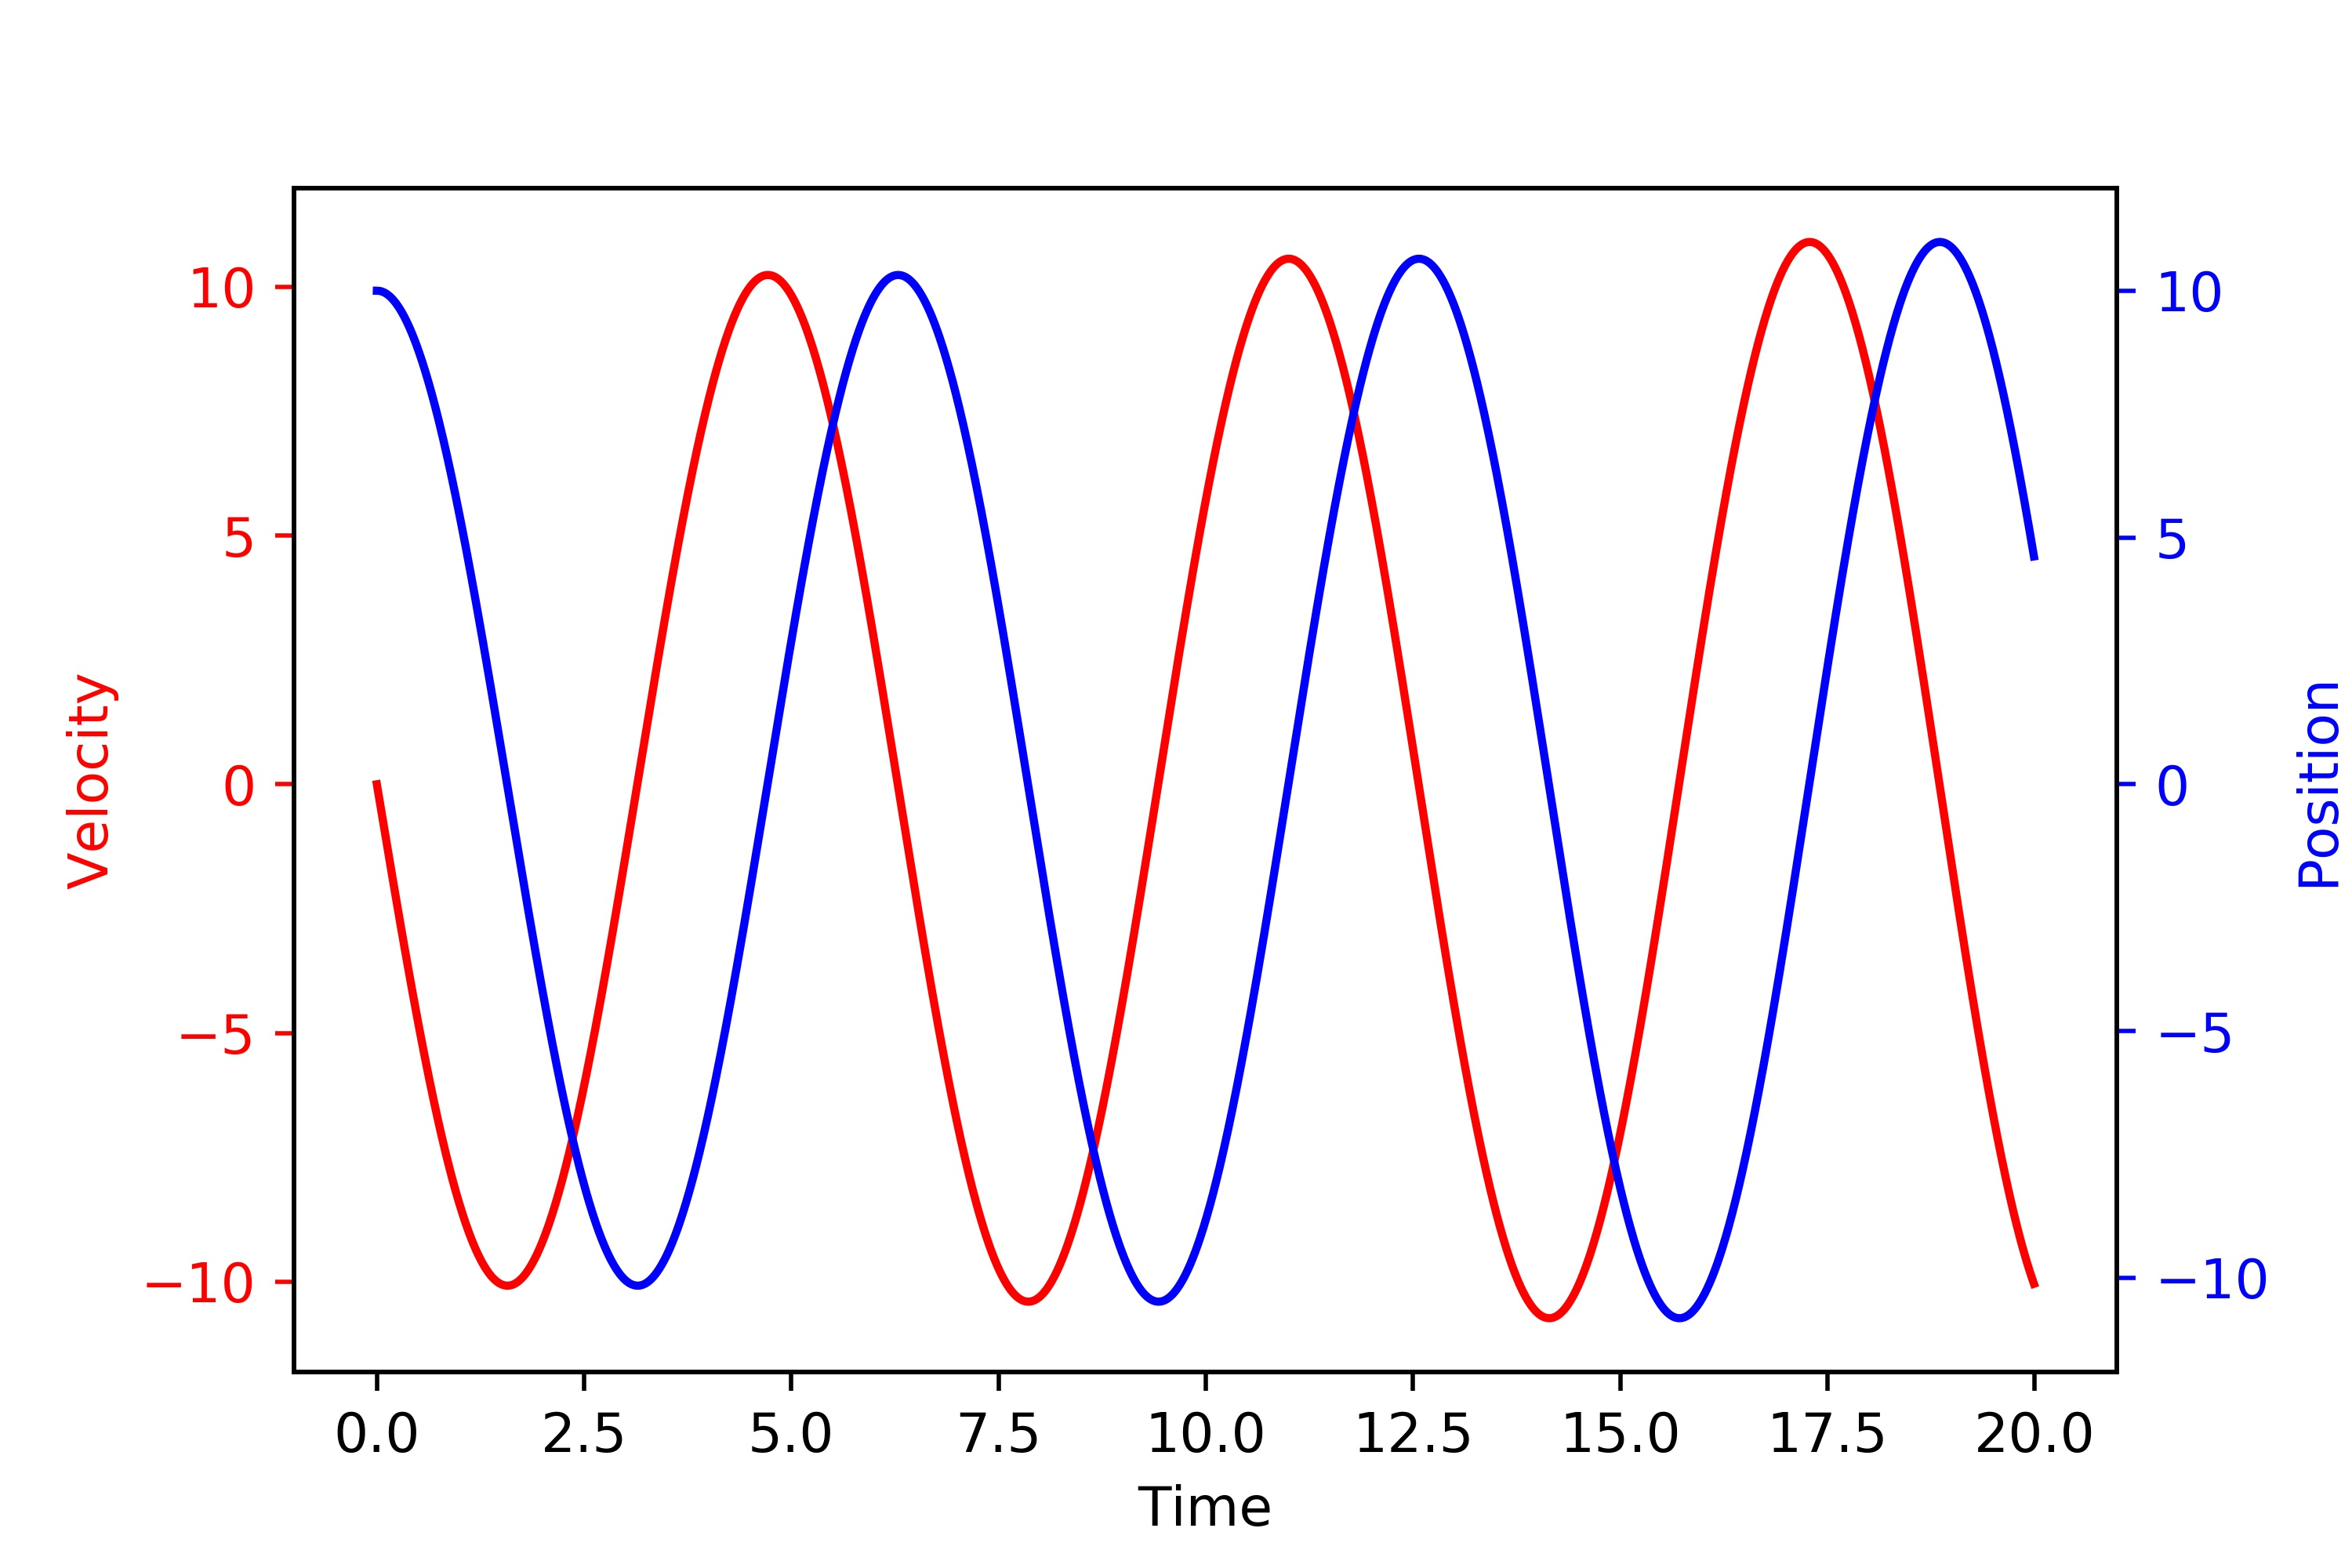
\includegraphics[width=\textwidth]{TVP1.jpg}
\caption{Position (blue) and velocity (red) plotted over time for a simple harmonic oscillator where $\omega=1$, the initial position is $x_0 = 10$, and the initial velocity is $v_0 = 0$. The interval $h$ used in the explicit Euler method was chosen to be 0.01.}
\end{figure}

\begin{figure}[H]
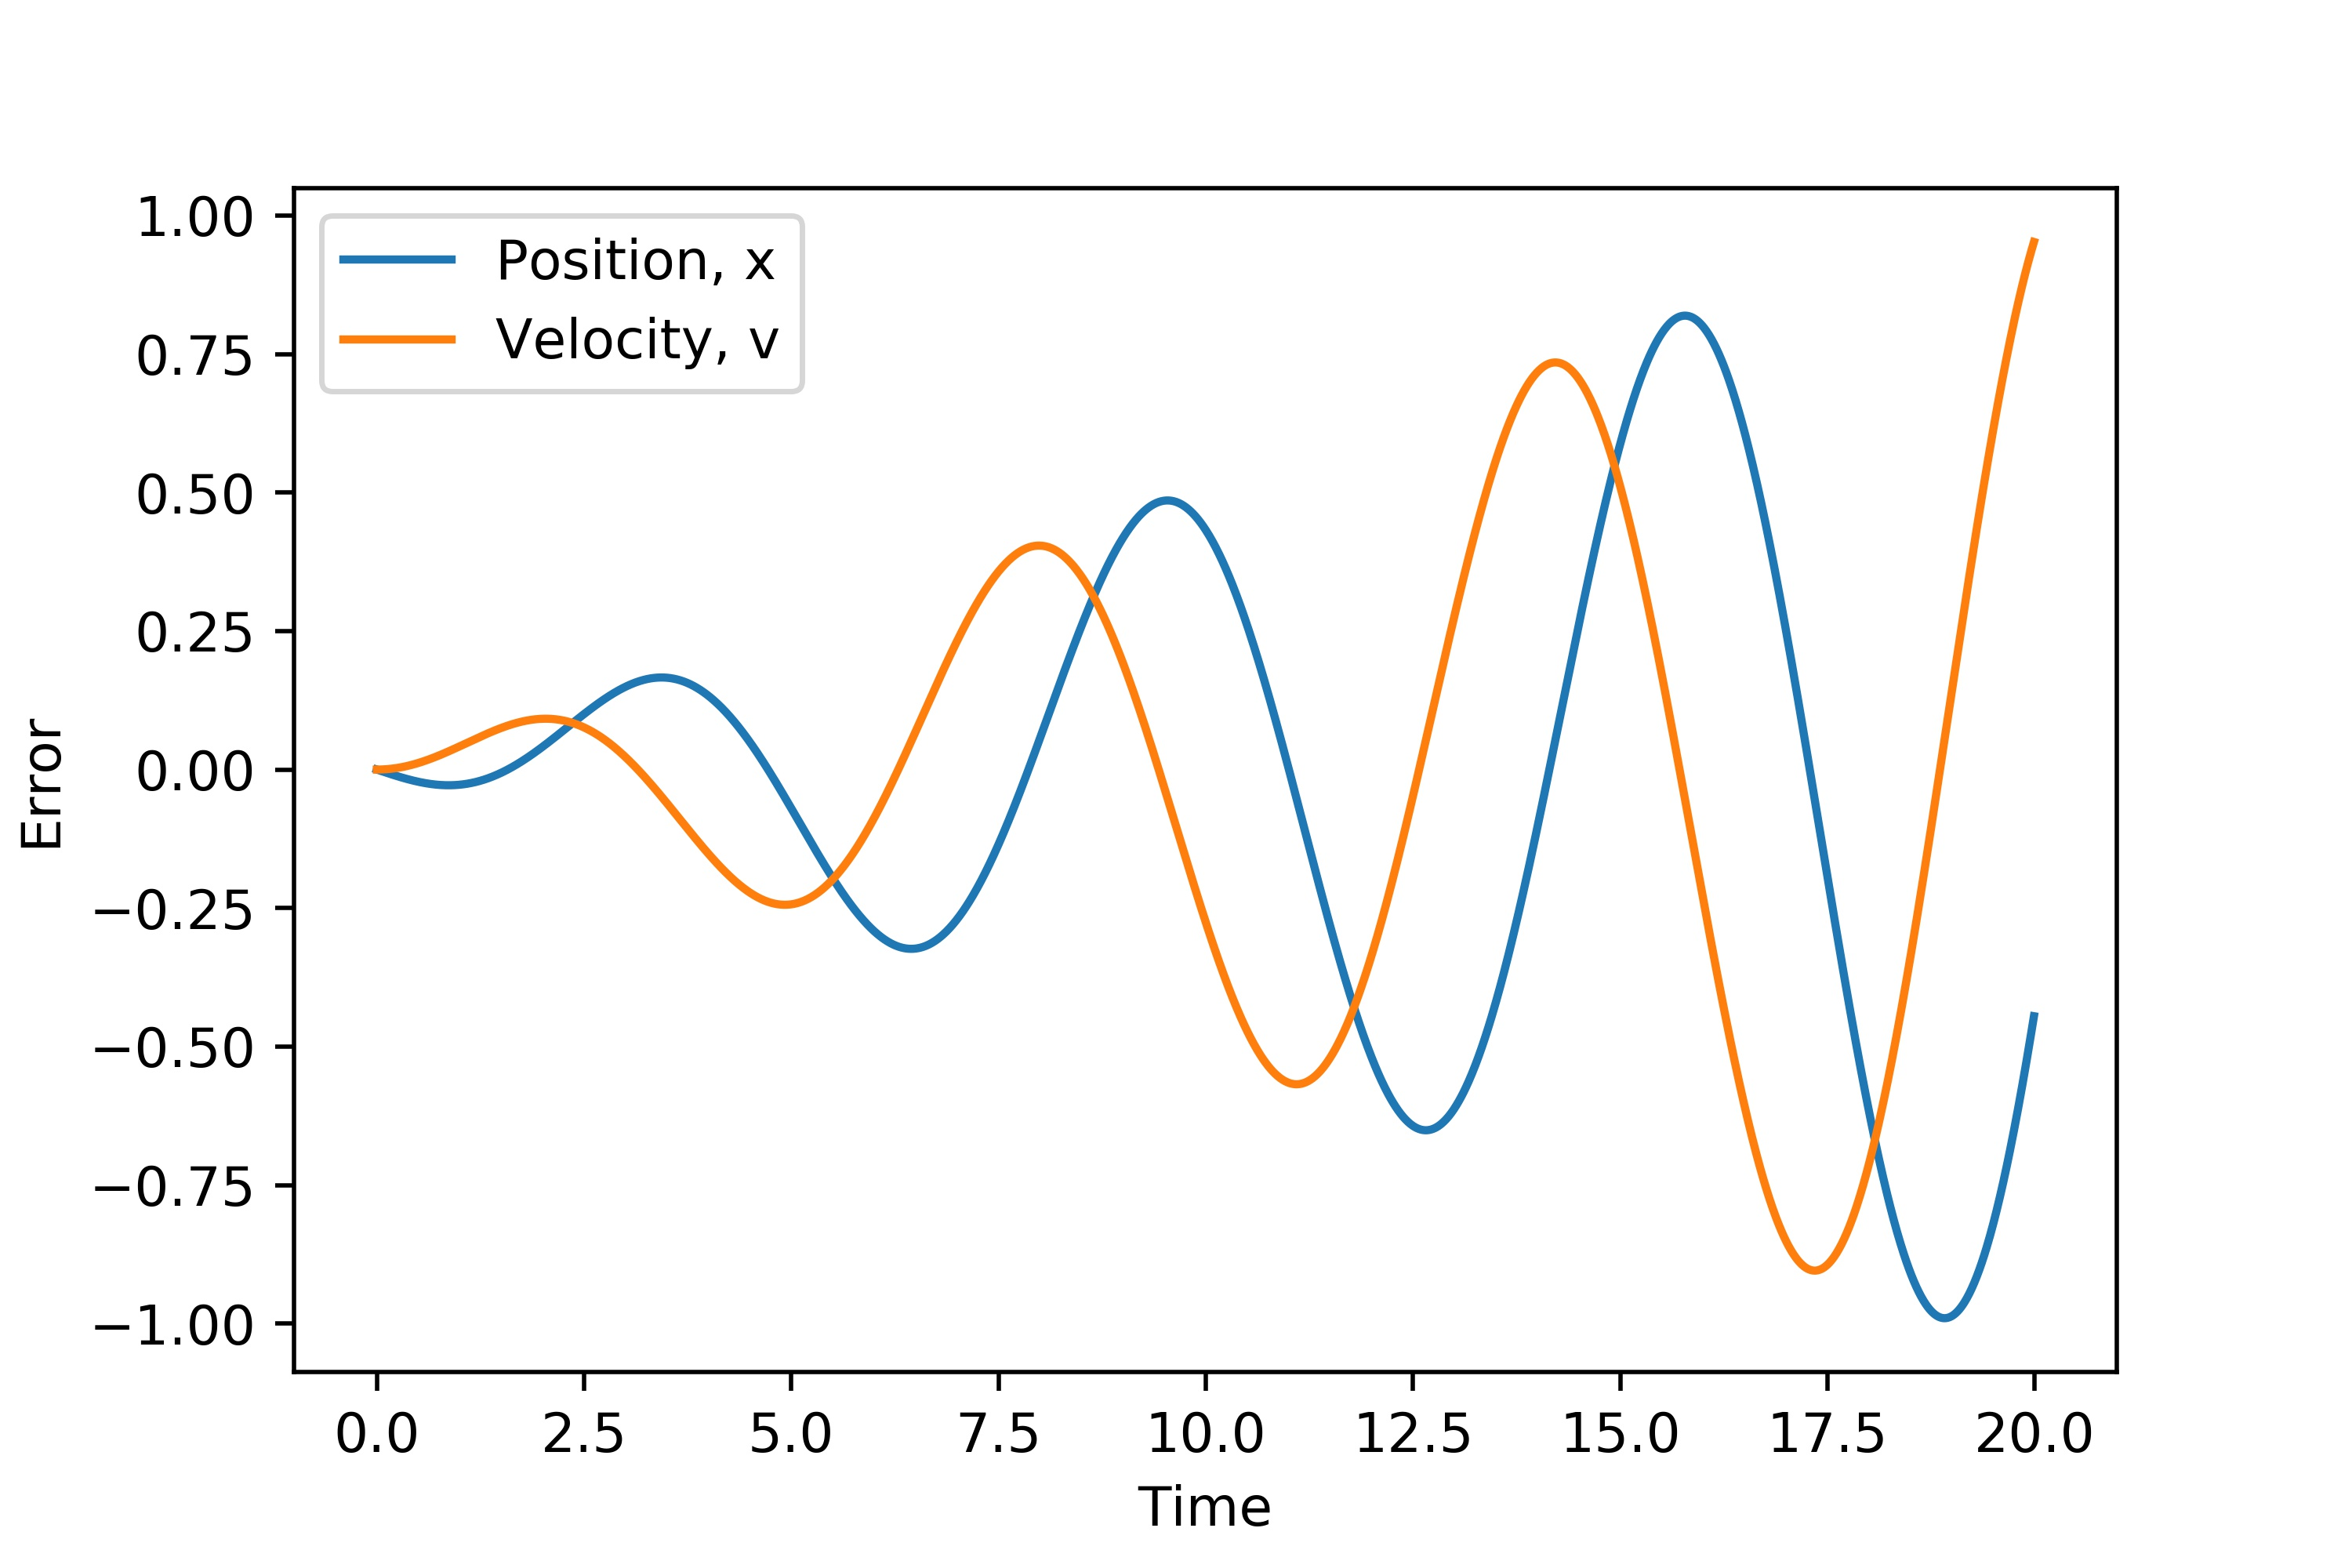
\includegraphics[width=\textwidth]{TErr1.jpg}
\caption{Absolute errors in the explicit numerical approximation of position (blue) and velocity (orange) as a function of time for the system and method described in Figure 1.}
\end{figure}

\begin{figure}[H]
\includegraphics[width=\textwidth]{HErr1.jpg}
\caption{Maximum error in the approximation of position between $t = 0$ and $t = 20$ as a function of the numerical interval $h$. Since $h$ is not small enough for roundoff error to be of concern, we conclude that truncation error is lienar in $h$ for reasonably small $h$.}
\end{figure}

\begin{figure}[H]
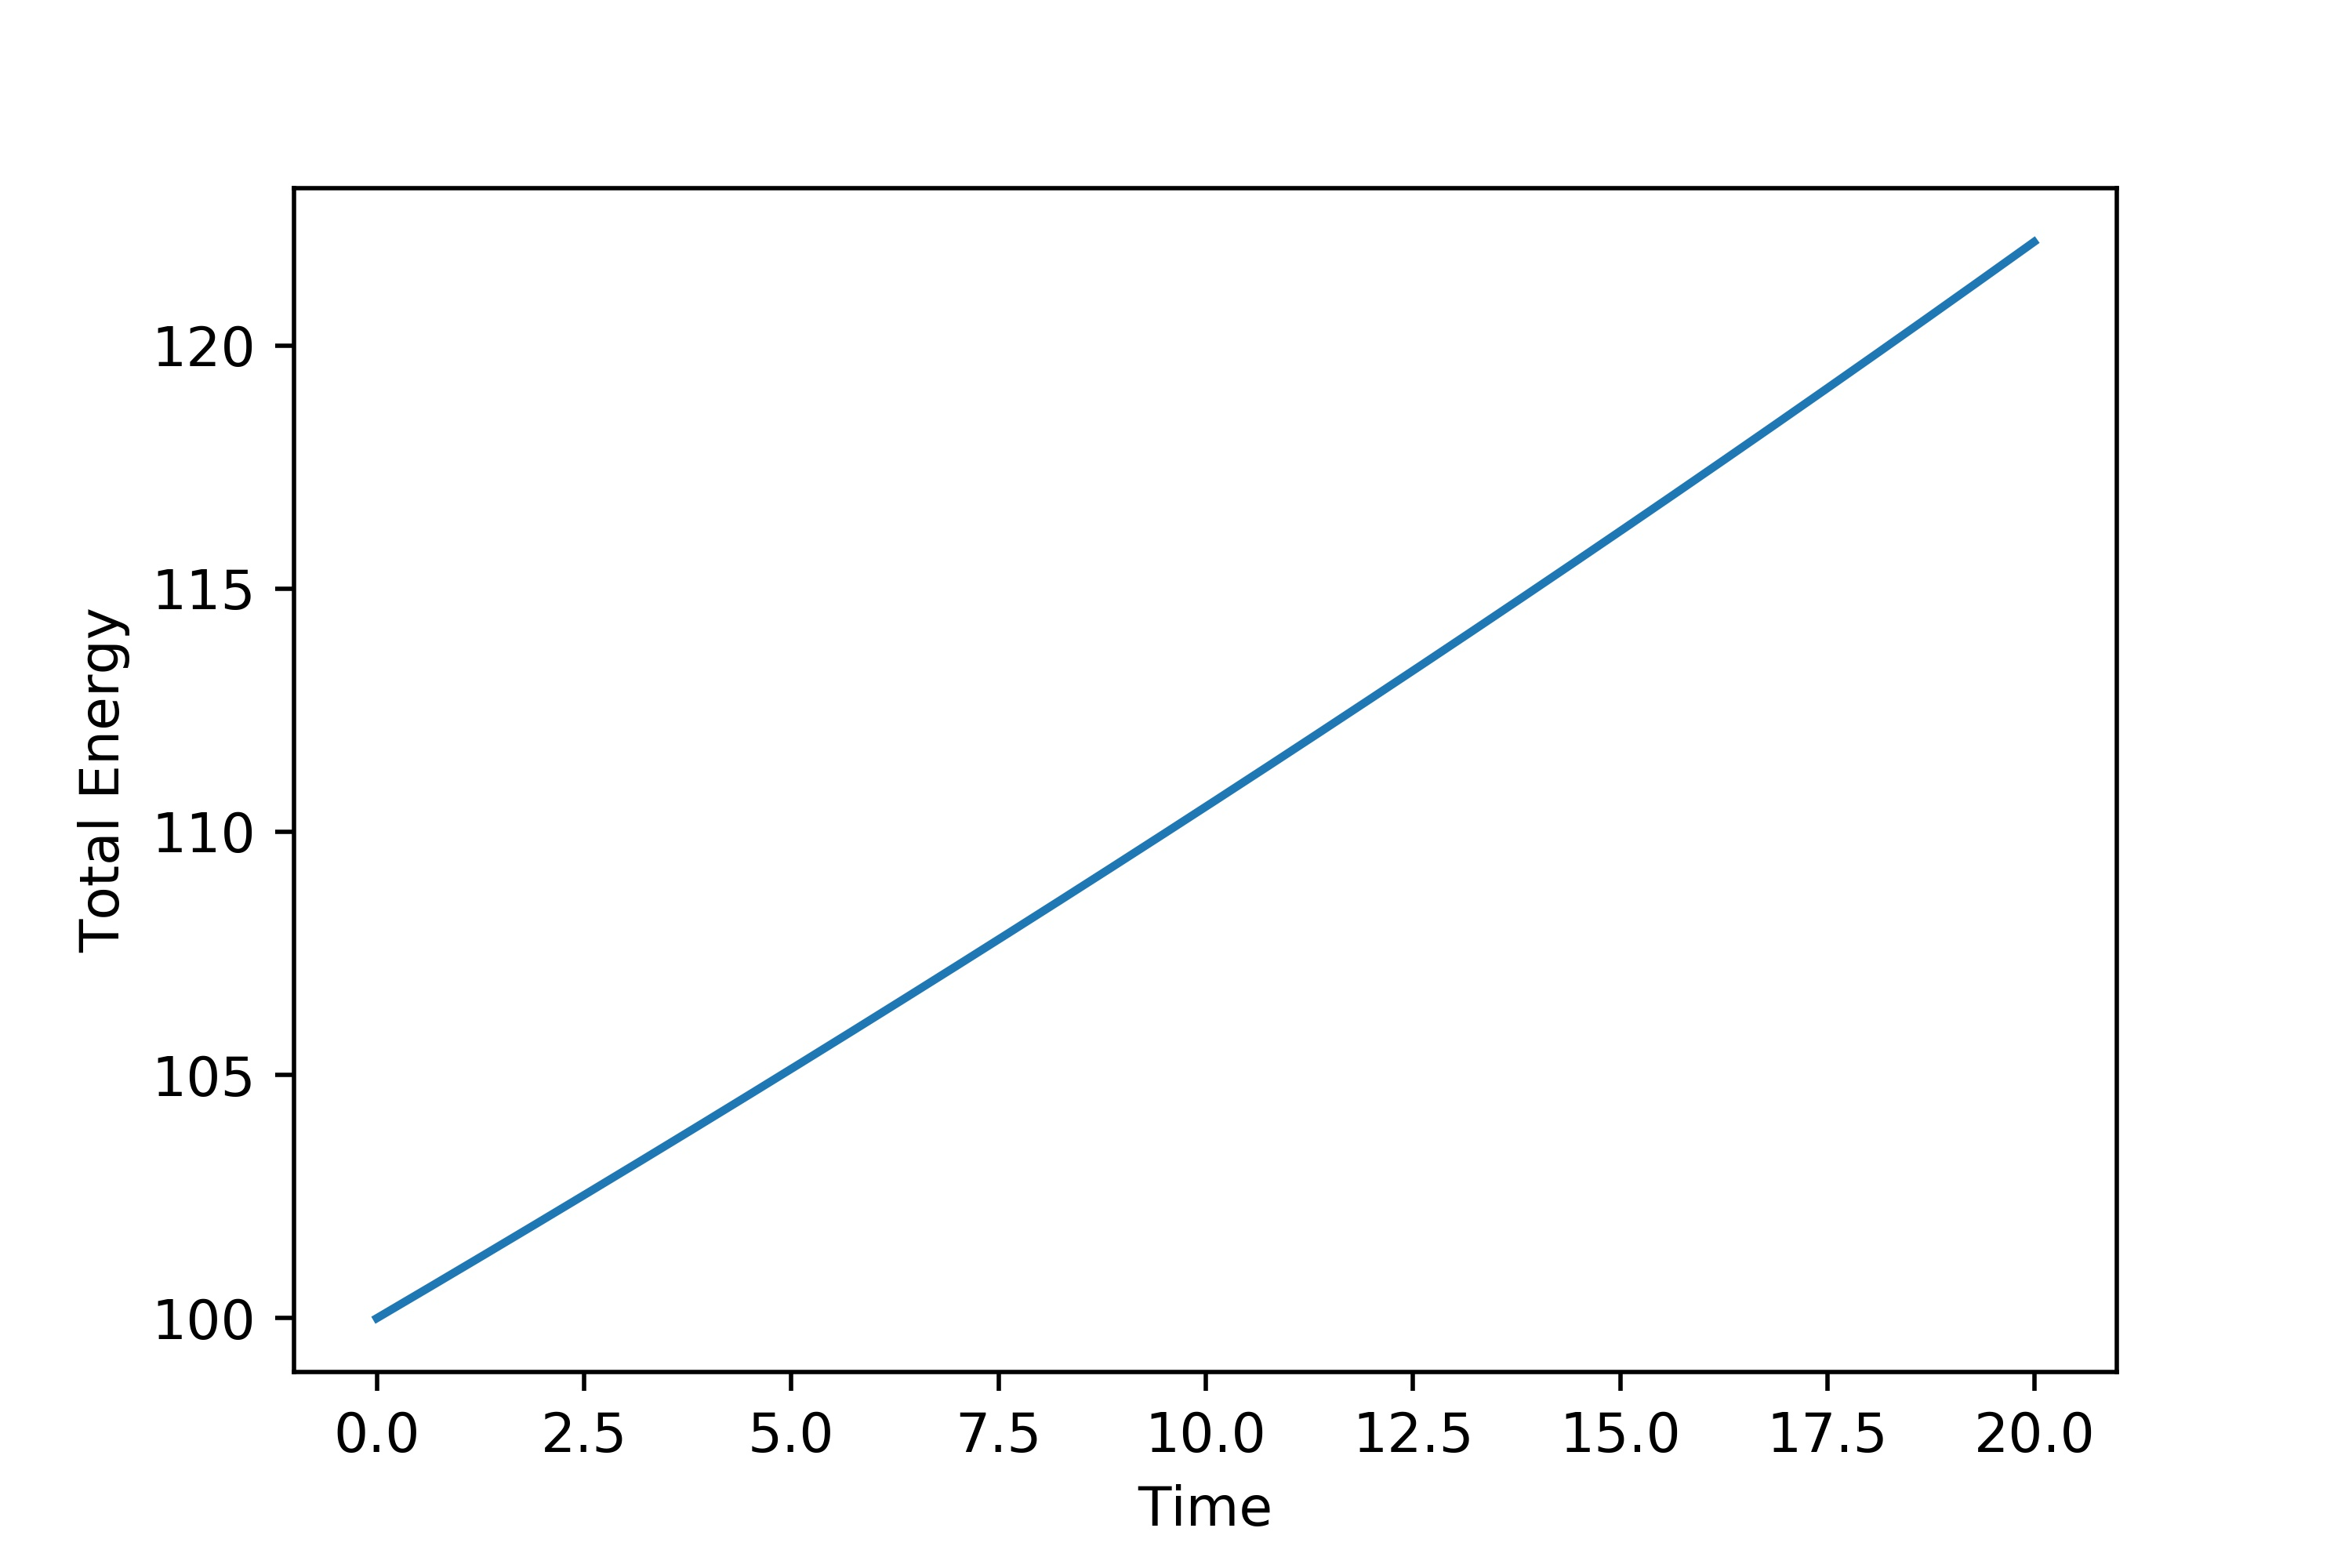
\includegraphics[width=\textwidth]{TE1.jpg}
\caption{Normalized total energy ($E = x^2 + v^2$ as a function of time for the numerical system described in Figure 1. The total energy evolves linearly over time, which suggests that even though the maximum deviations of position and velocity of the oscillator scale linearly over time (see Figure 2), the maximum allowed amplitude must scale at a slower pace ($\sim \sqrt{x}$).}
\end{figure}

\section{Implicit Euler Formula}

\begin{figure}[H]
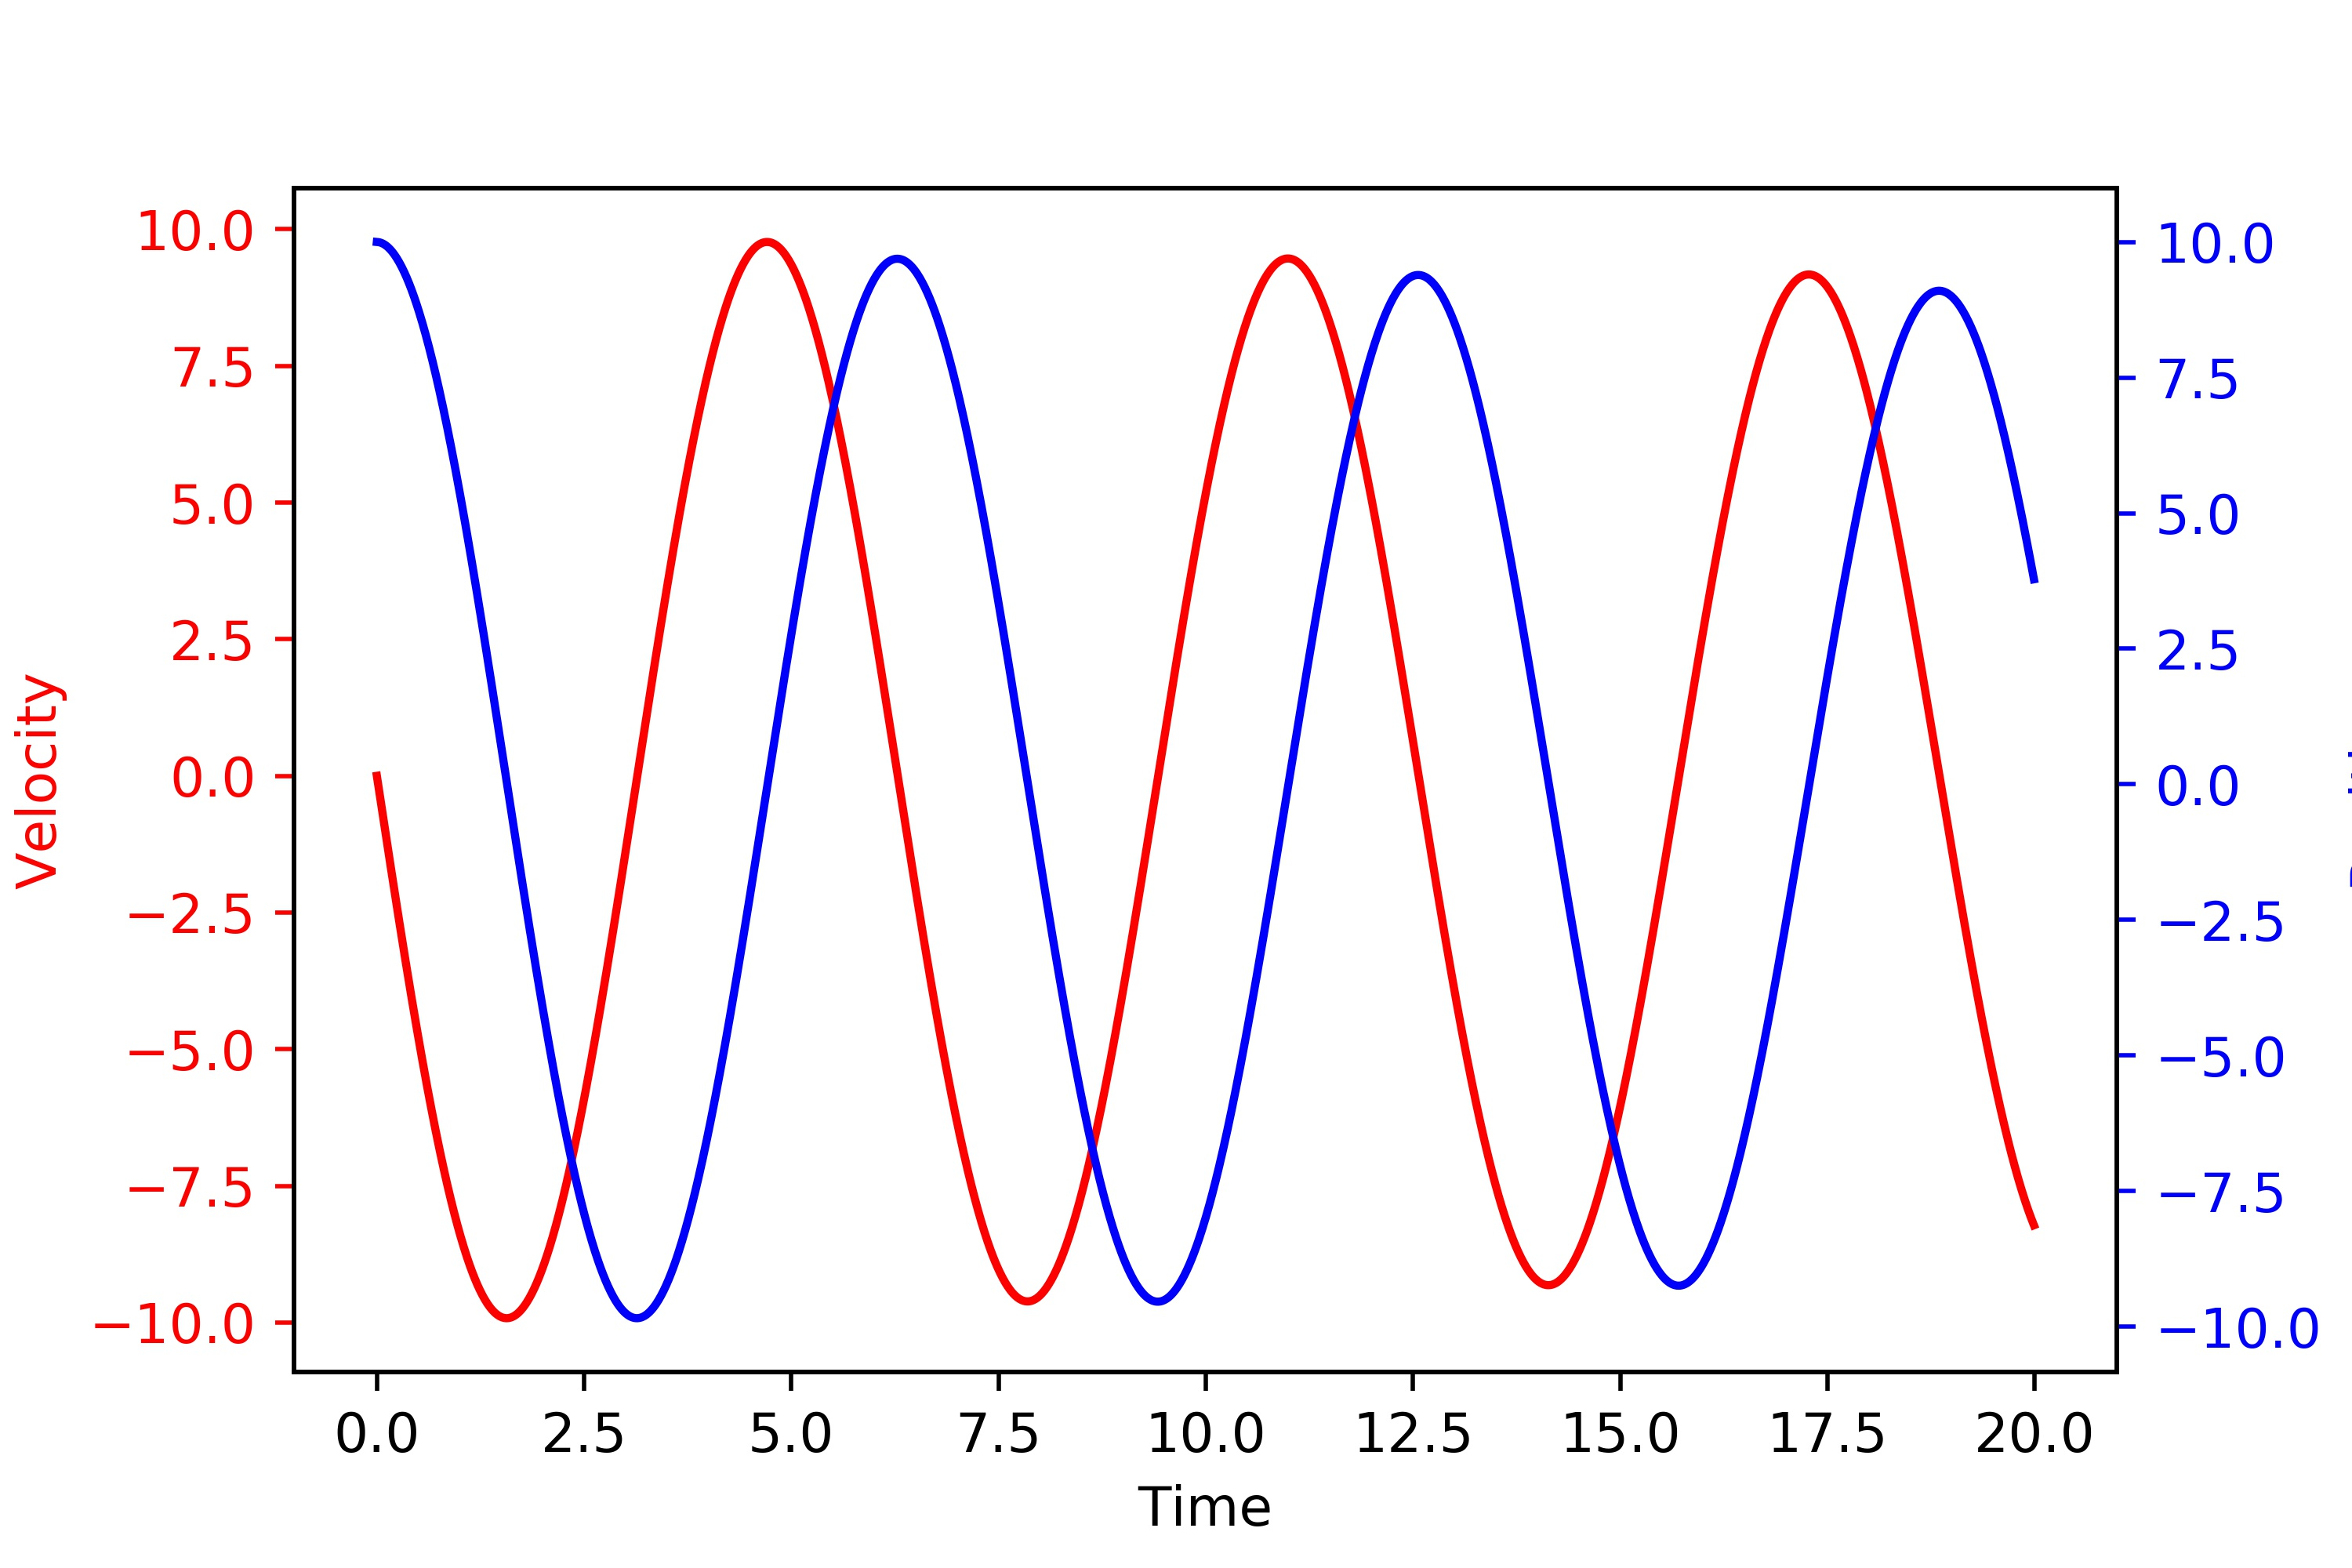
\includegraphics[width=\textwidth]{TVP2.jpg}
\caption{Position (blue) and velocity (red) plotted over time for a simple harmonic oscillator where $\omega=1$, the initial position is $x_0 = 10$, and the initial velocity is $v_0 = 0$. The interval $h$ used for the (now implicit) Euler method was chosen to be 0.01. Unlike the explicit mechanism illustrated in Figure 1, the maximum amplitudes of position and velocity appear to be decreasing over time under the implicit Euler formalism.}
\end{figure}

\begin{figure}[H]
\includegraphics[width=\textwidth]{Terr2.jpg}
\caption{Absolute errors in the implicit numerical approximation of position (blue) and velocity (orange) as a function of time for the system described in Figure 1. The errors associated with these parameters appear to be roughly 180$^\circ$ out of sync with but similar in magnitude to the errors achieved via the explicit formalism (see Figure 2).}
\end{figure}
\begin{figure}[H]
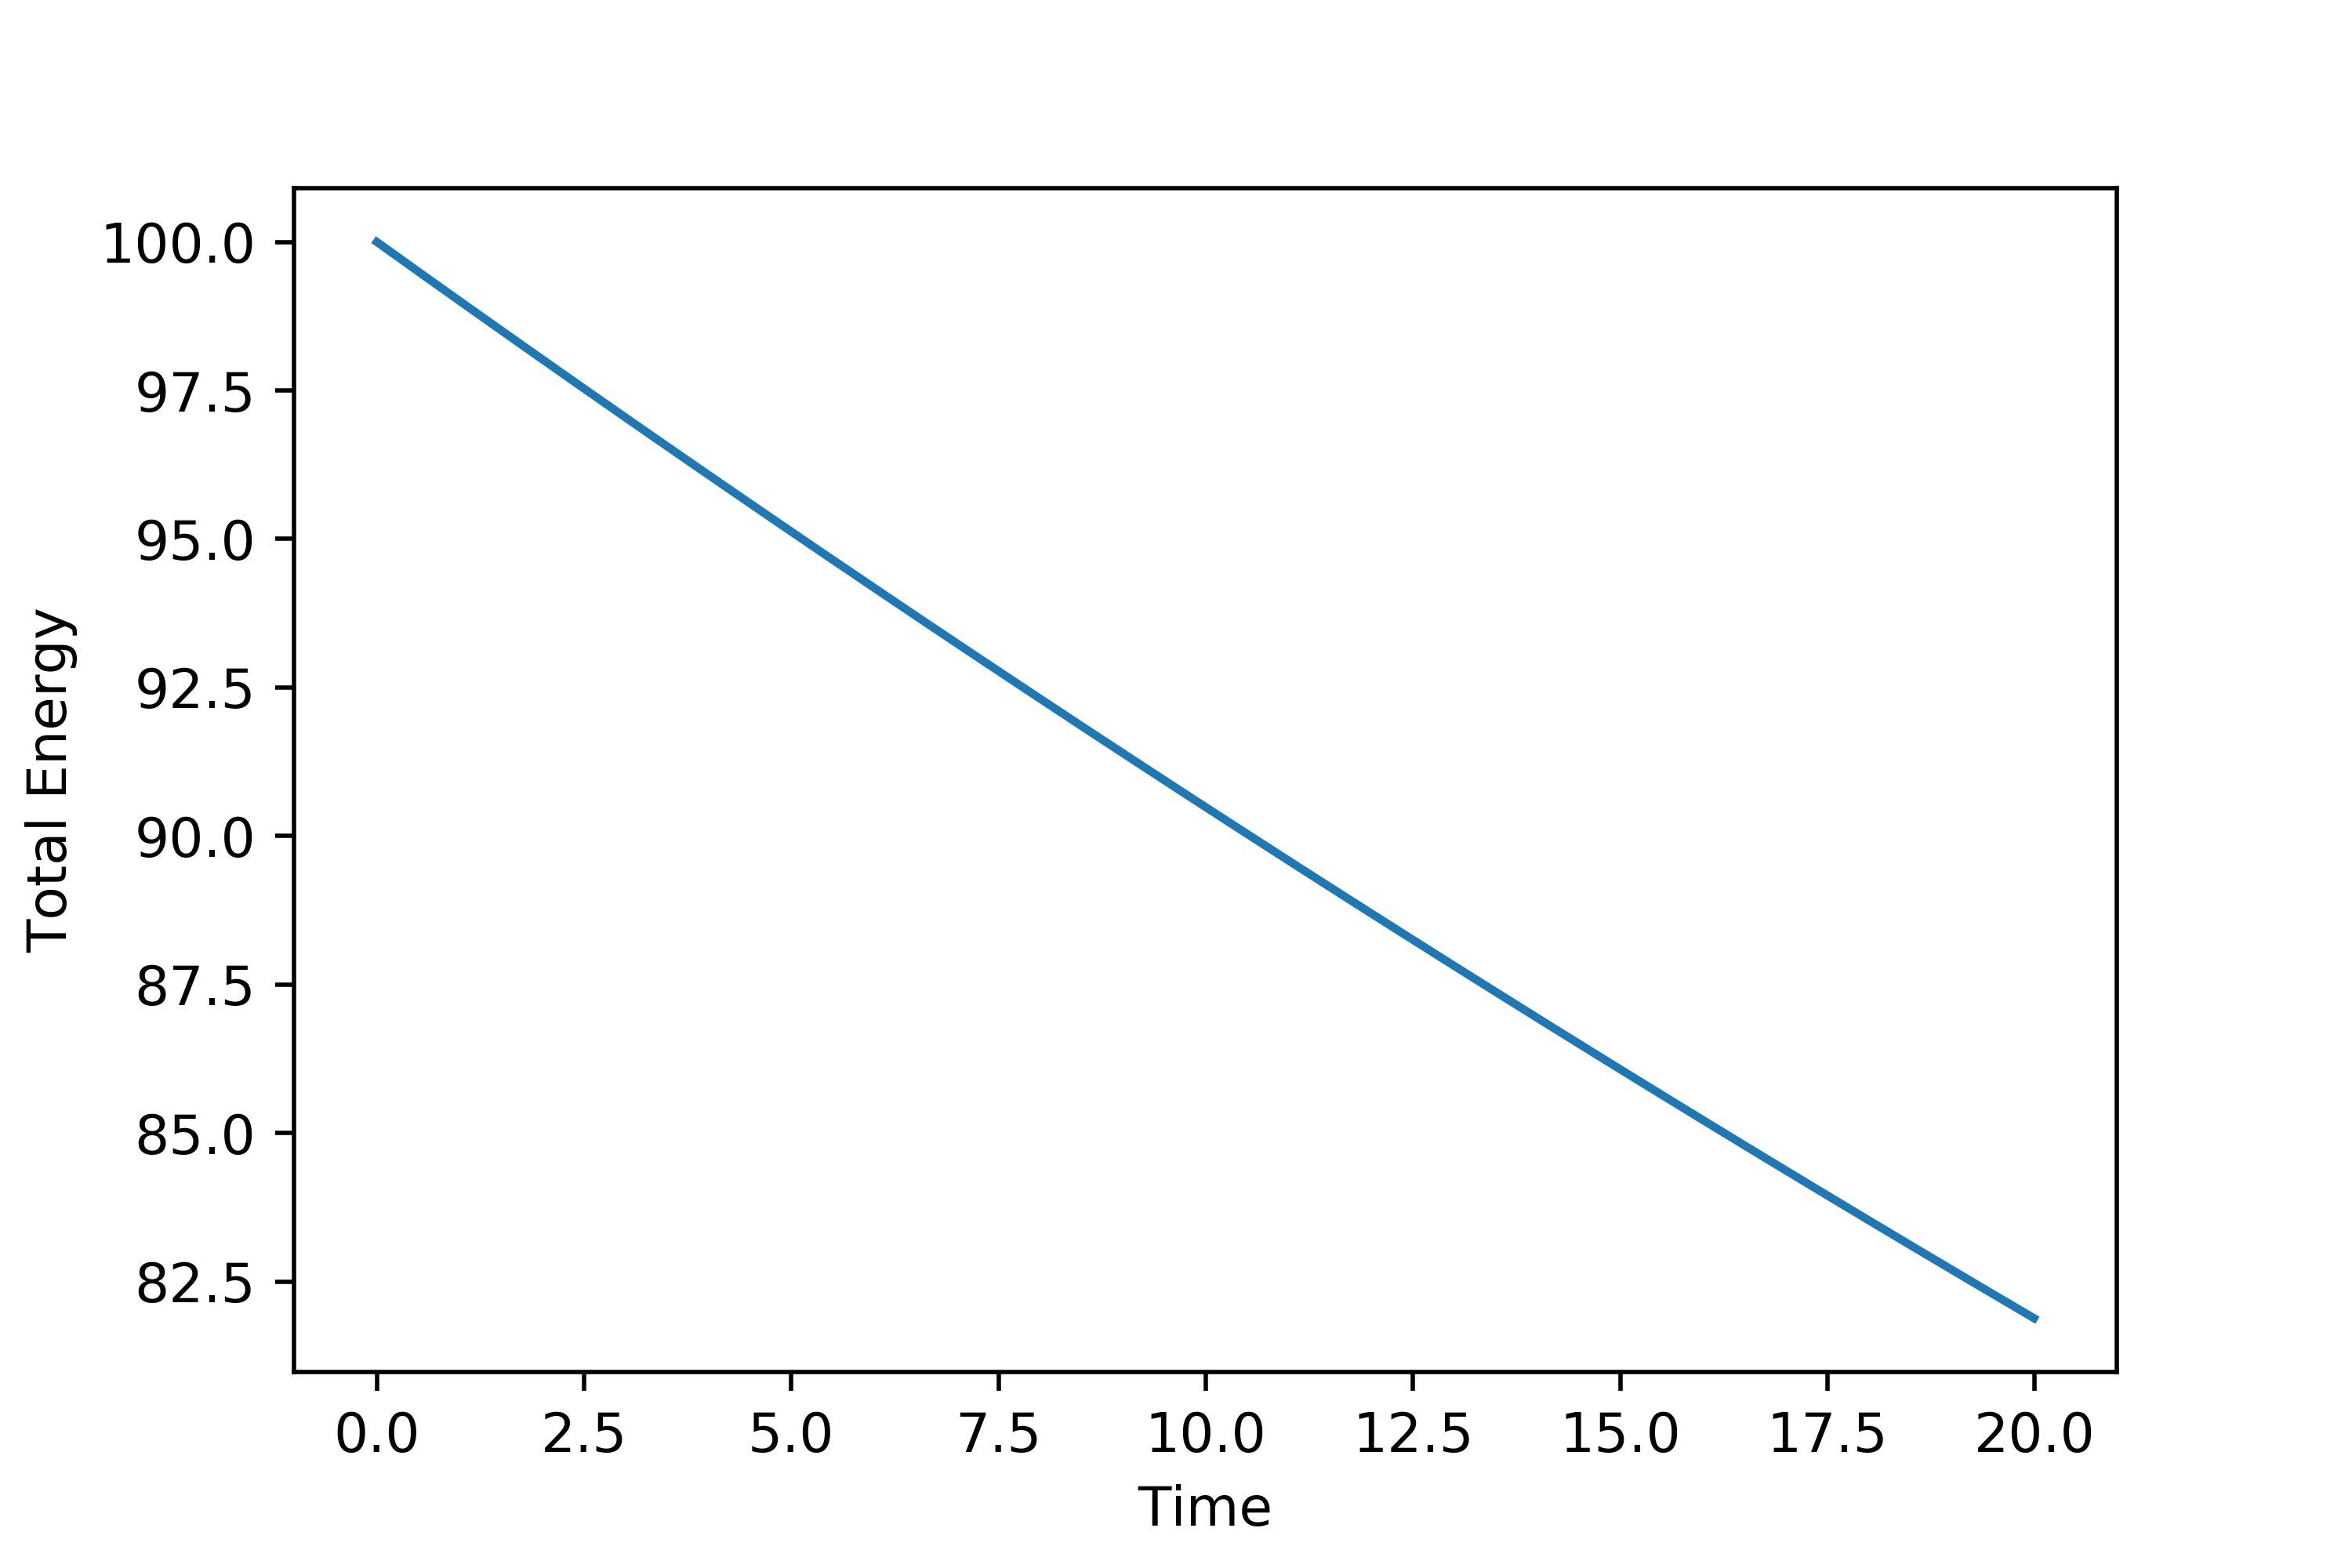
\includegraphics[width=\textwidth]{TE2.jpg}
\caption{Normalized total energy ($E = x^2 + v^2$ as a function of time for the numerical system described in Figure 1. The total energy again evolves linearly over time, but this time with a negative derivative.}
\end{figure}

\section{Phase Space Geometry \& Symplectic Euler Method}

\begin{figure}[H]
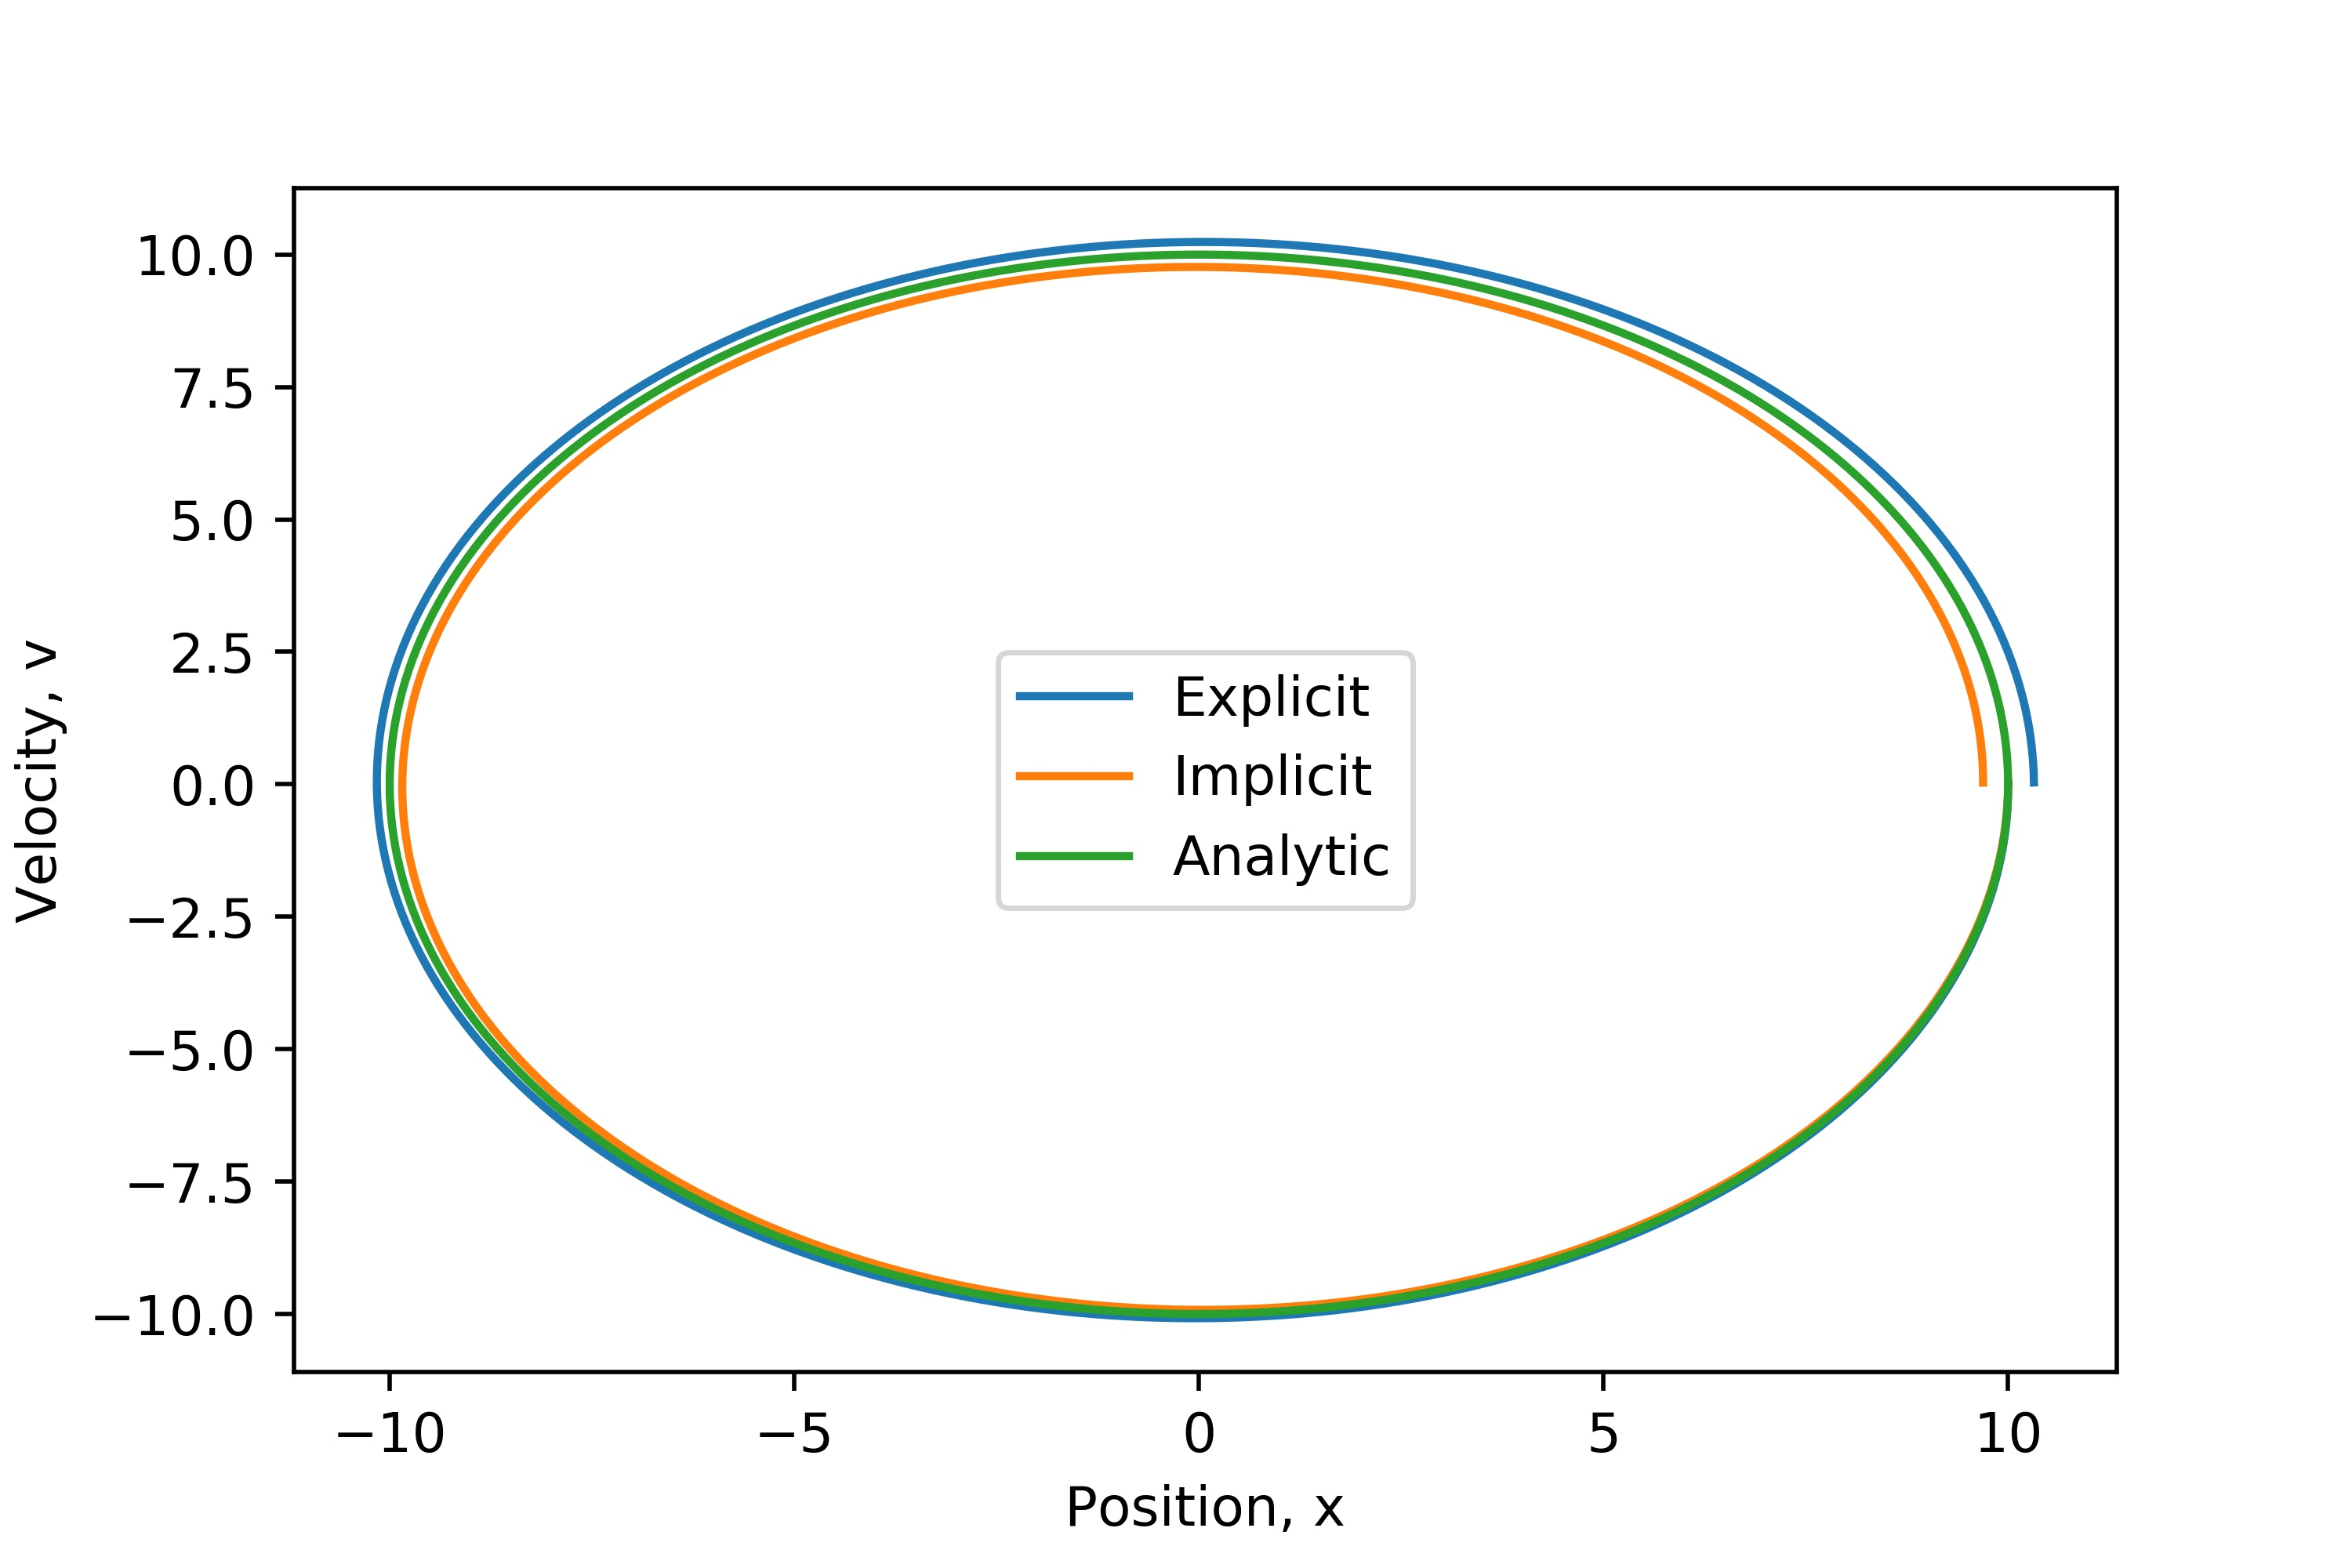
\includegraphics[width=\textwidth]{phase1.jpg}
\caption{Phase-space geometries of the trajectories produced by the explicit (blue), implicit (orange), and analytic (green) representations of the simple harmonic oscillator. Over time, the explicitly modeled oscillator gains energy and thus draws contours around the analytic oscillator, while the implicitly modeled one loses energy and spirals inward toward $x = v = 0$.}
\end{figure}

\begin{figure}[H]
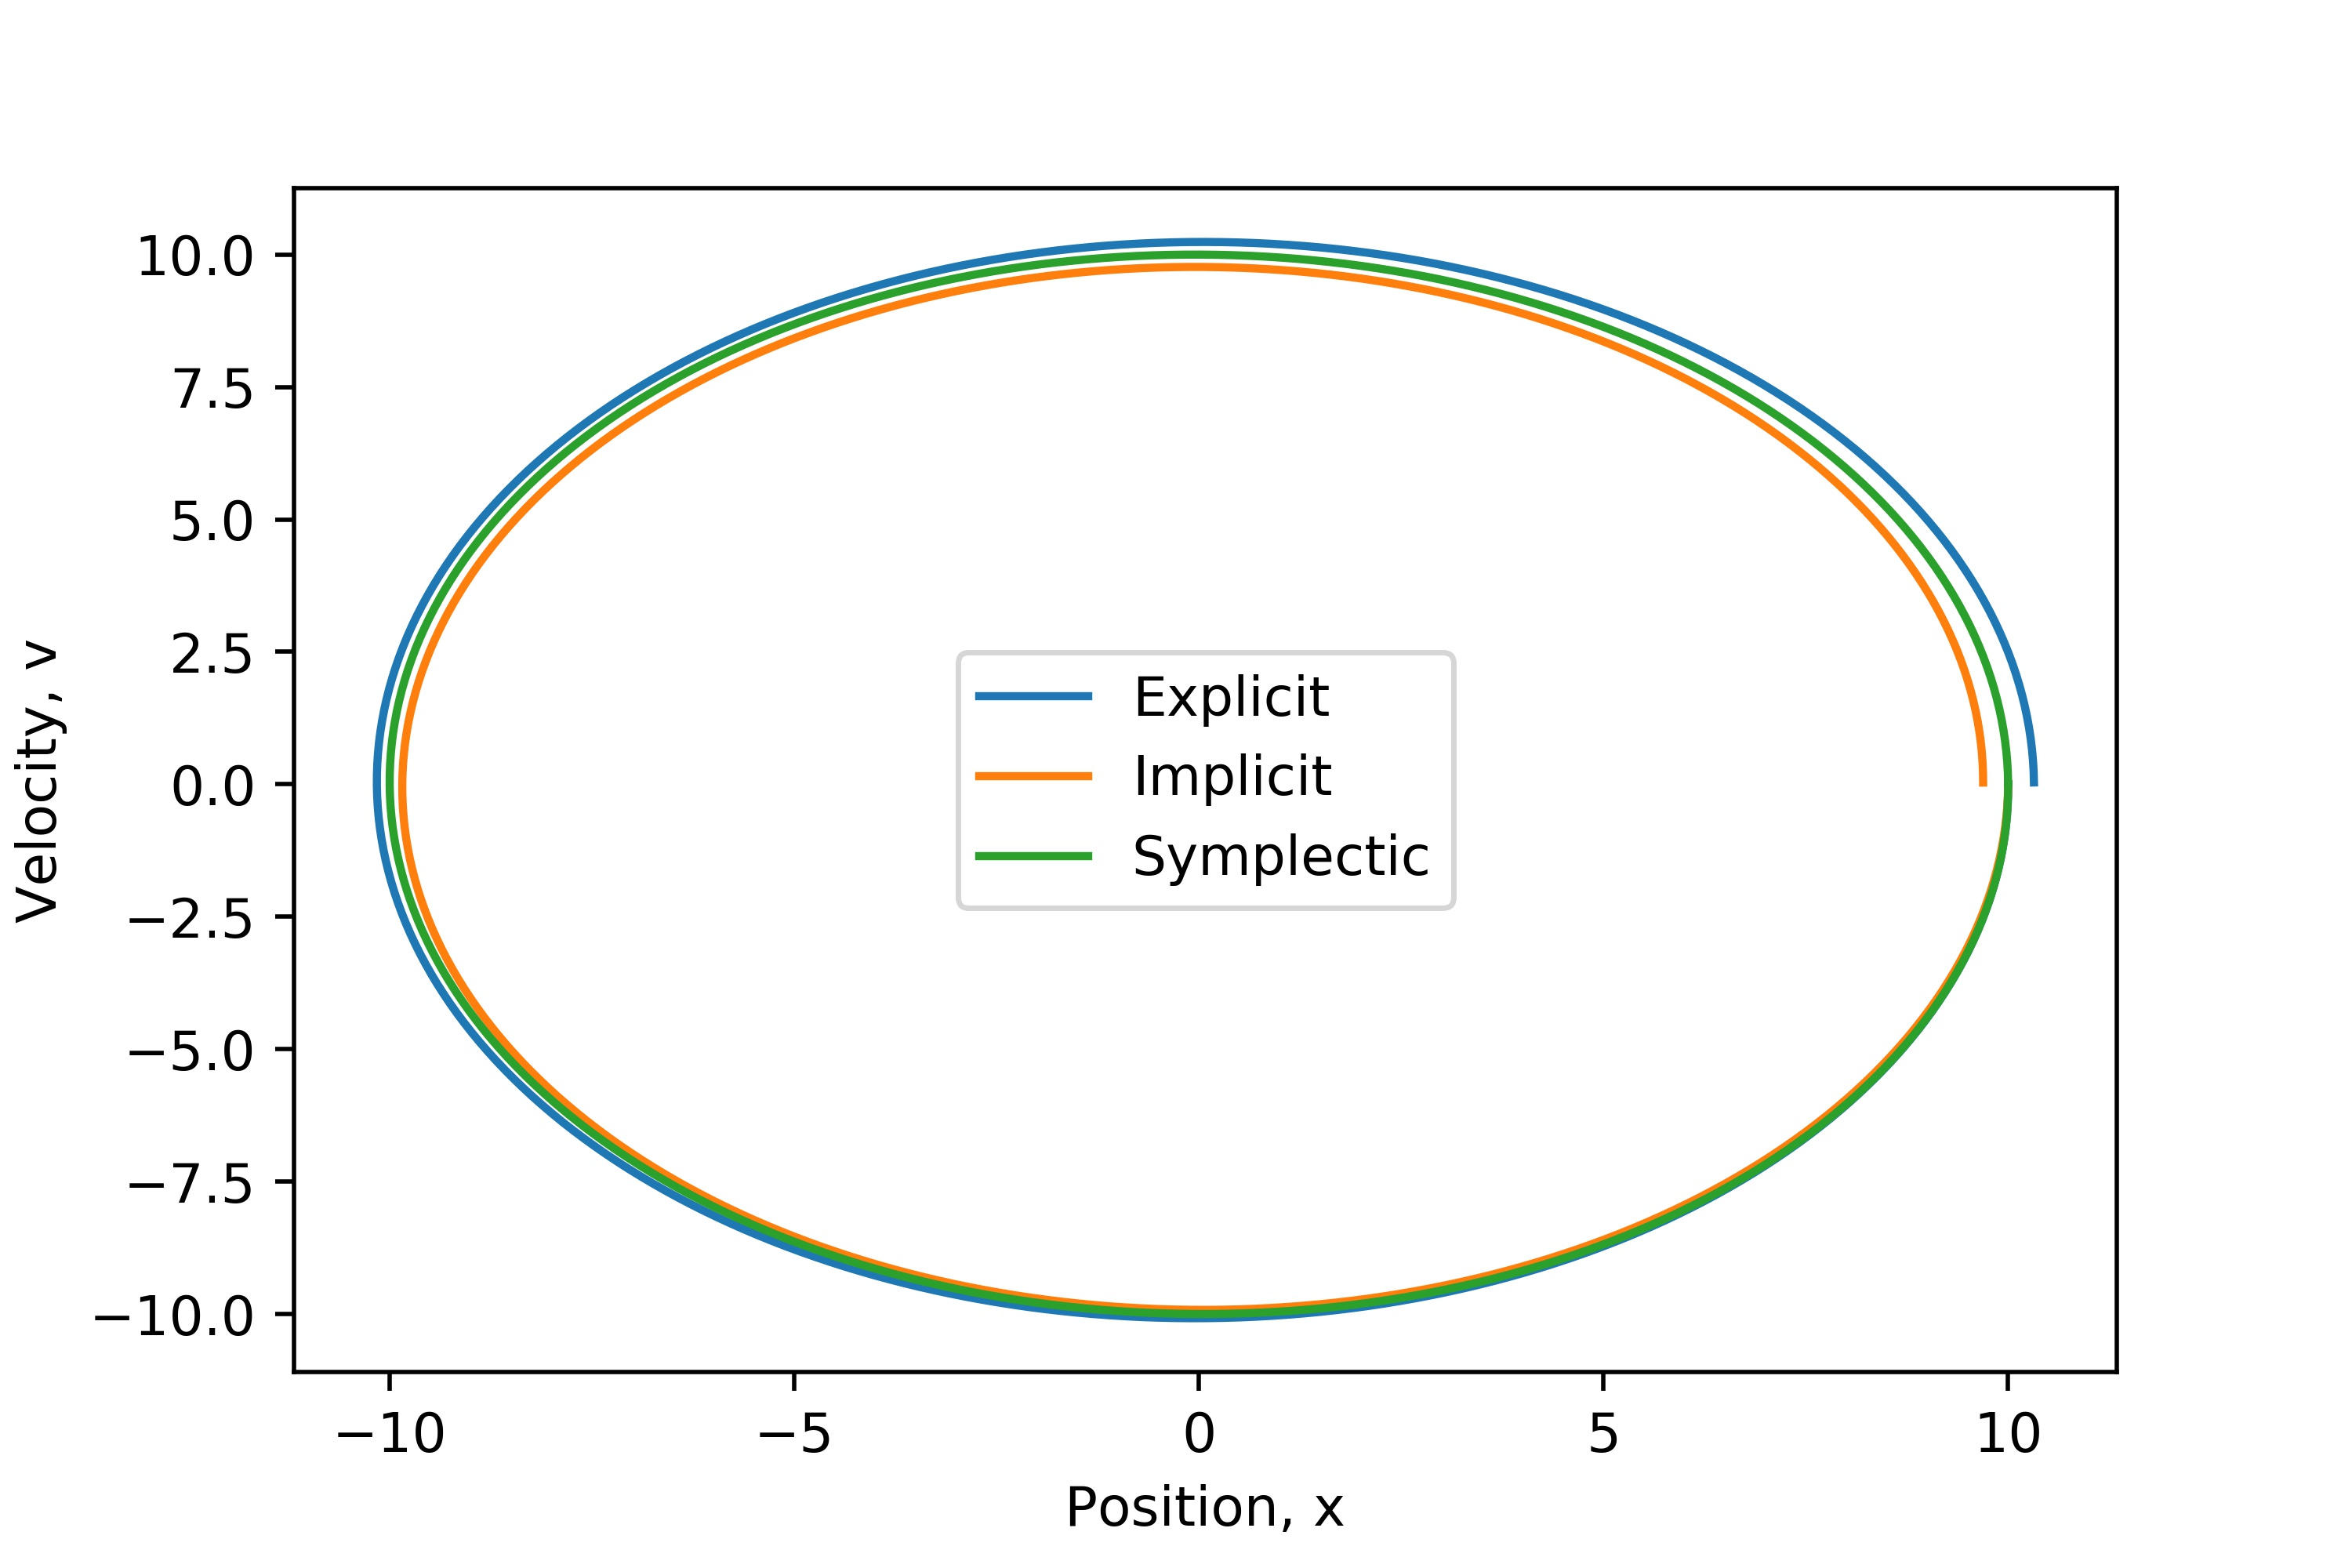
\includegraphics[width=\textwidth]{phase2.jpg}
\caption{Phase-space geometry of the symplectically modeled oscillator relative to explicit and implicit Euler methods. The symplectic model is reminiscent of the analytic phase-space structure presented in Figure 8 for small h, in that is forms a closed loop in between the explicit and implicit curves.}
\end{figure}

\begin{figure}[H]
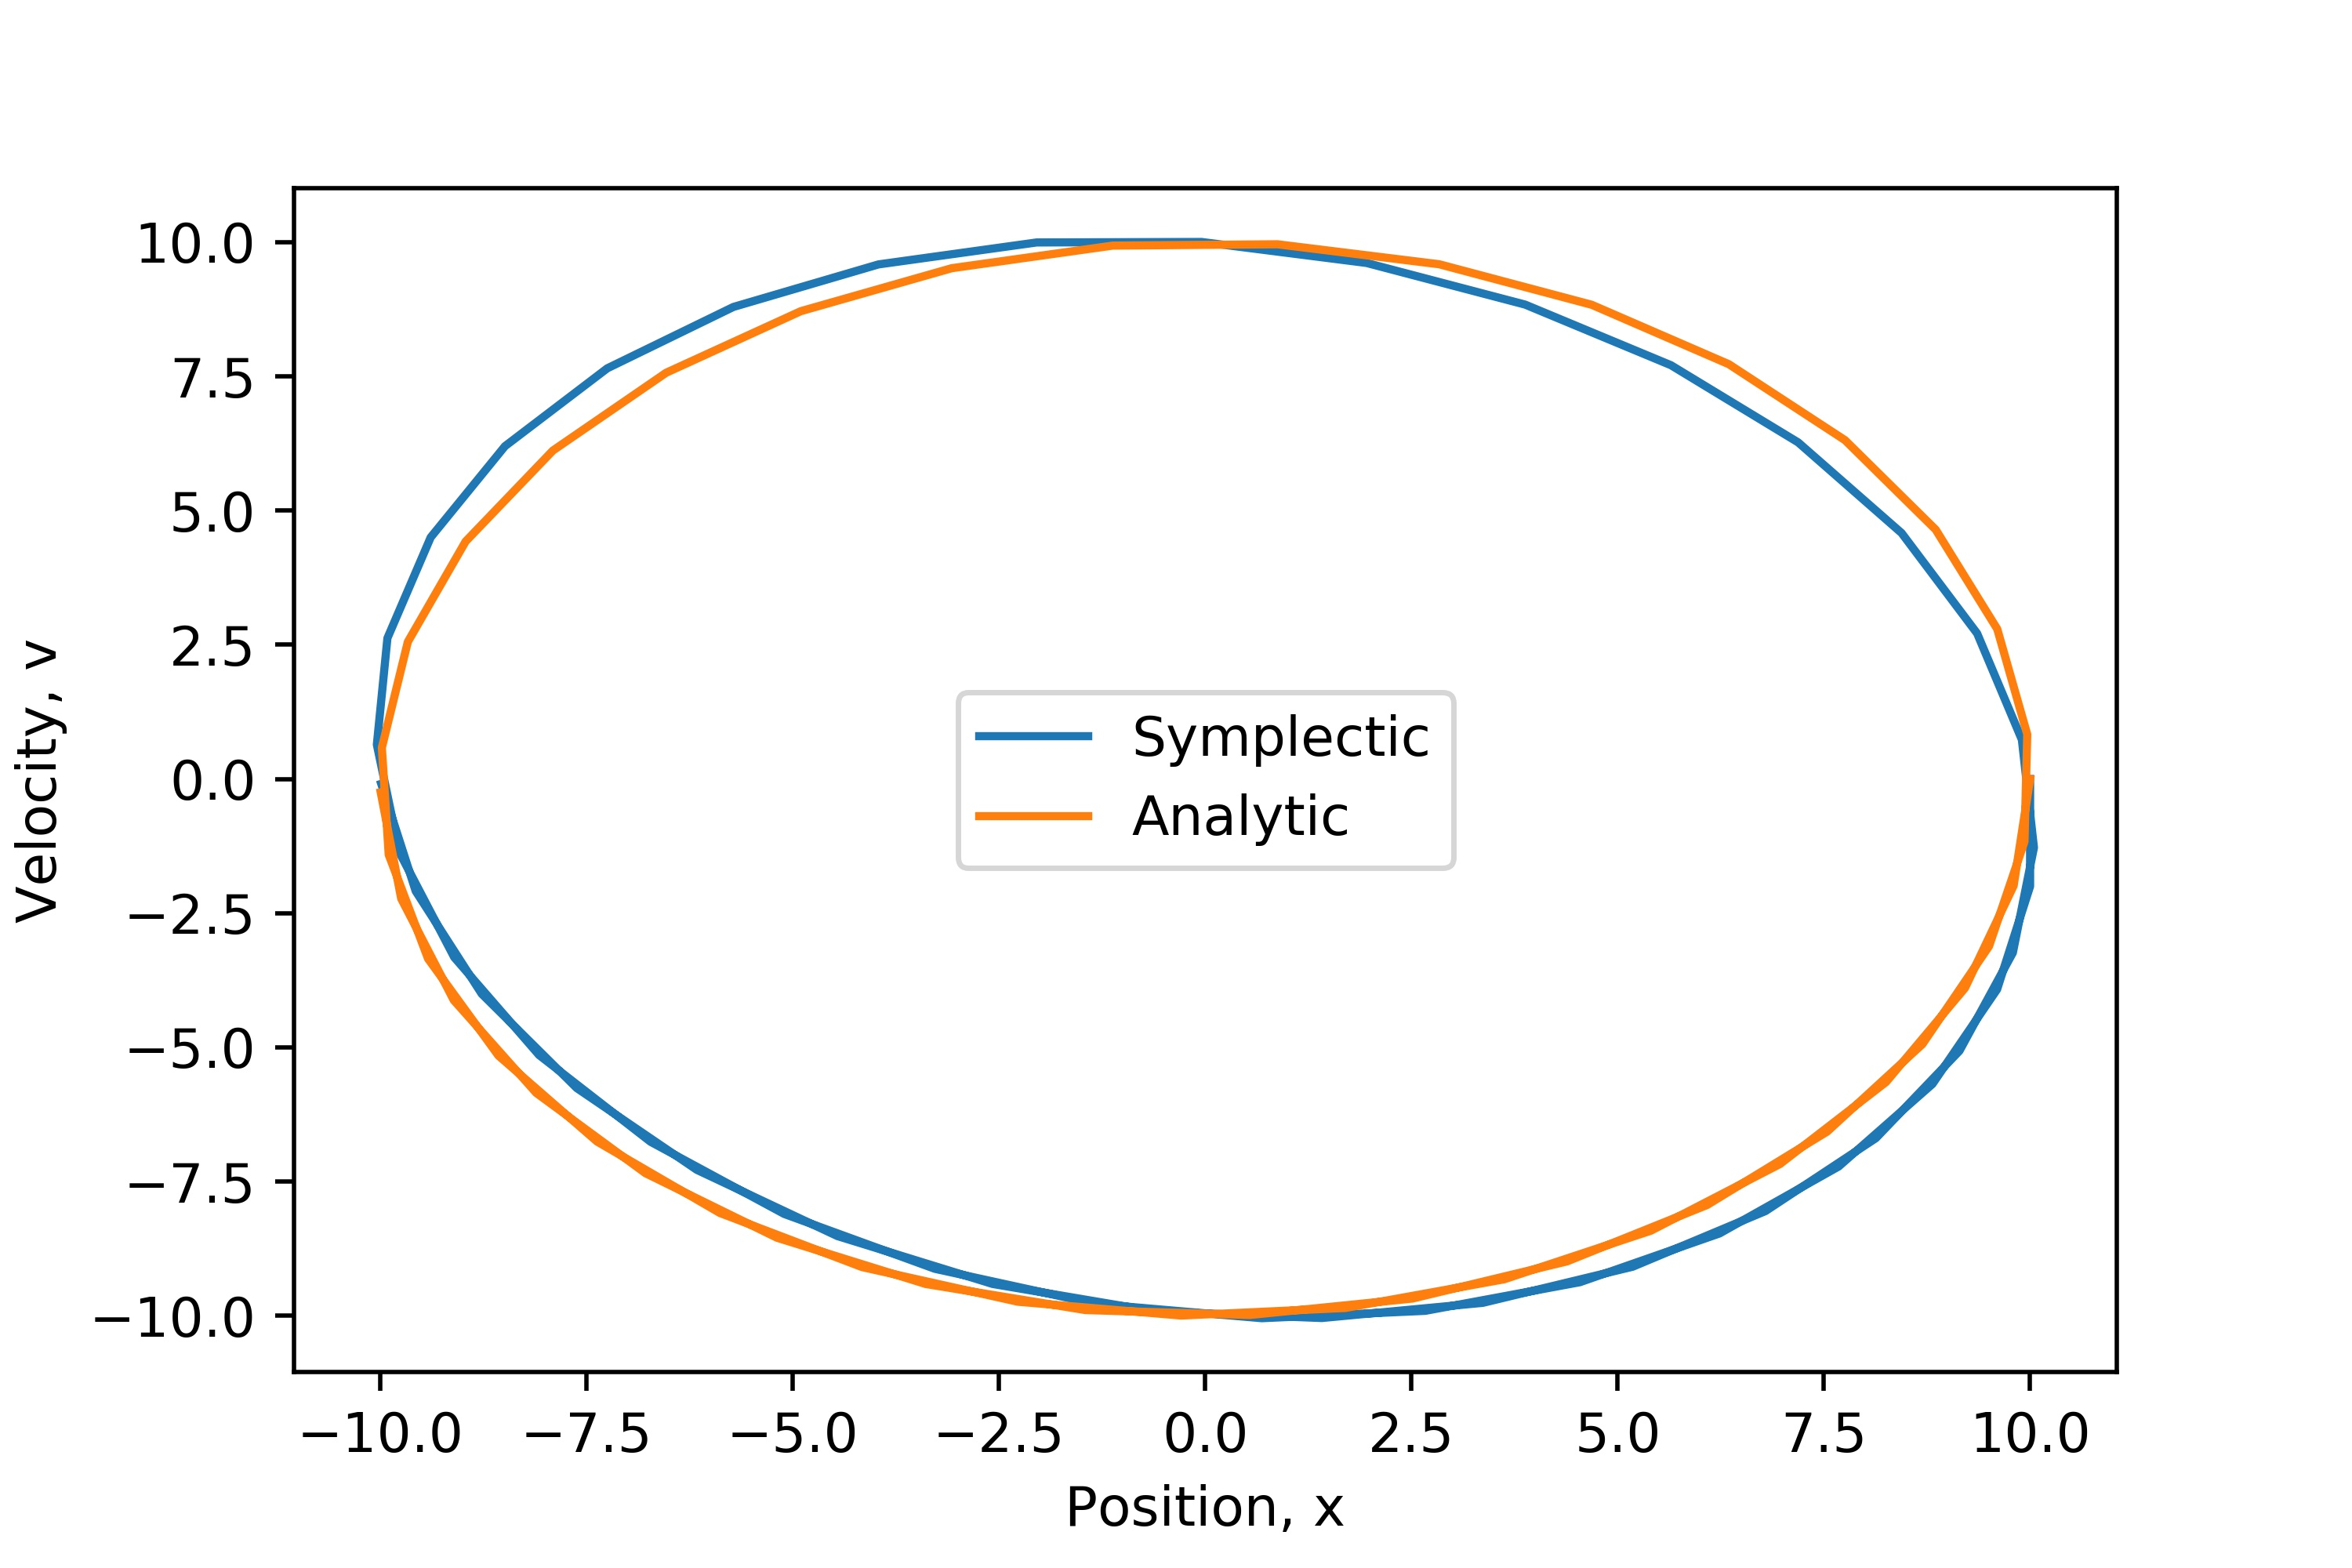
\includegraphics[width=\textwidth]{phase3.jpg}
\caption{Comparison of the symplectic model using a higher time interval $h$ (0.20) with a true analytic simple harmonic oscillator. Unlike the symplectic curve of Figure 9, the low-resolution symplectic model  is no longer perfectly circular, though the area, as promised, is kept constant.}
\end{figure}

\begin{figure}[H]
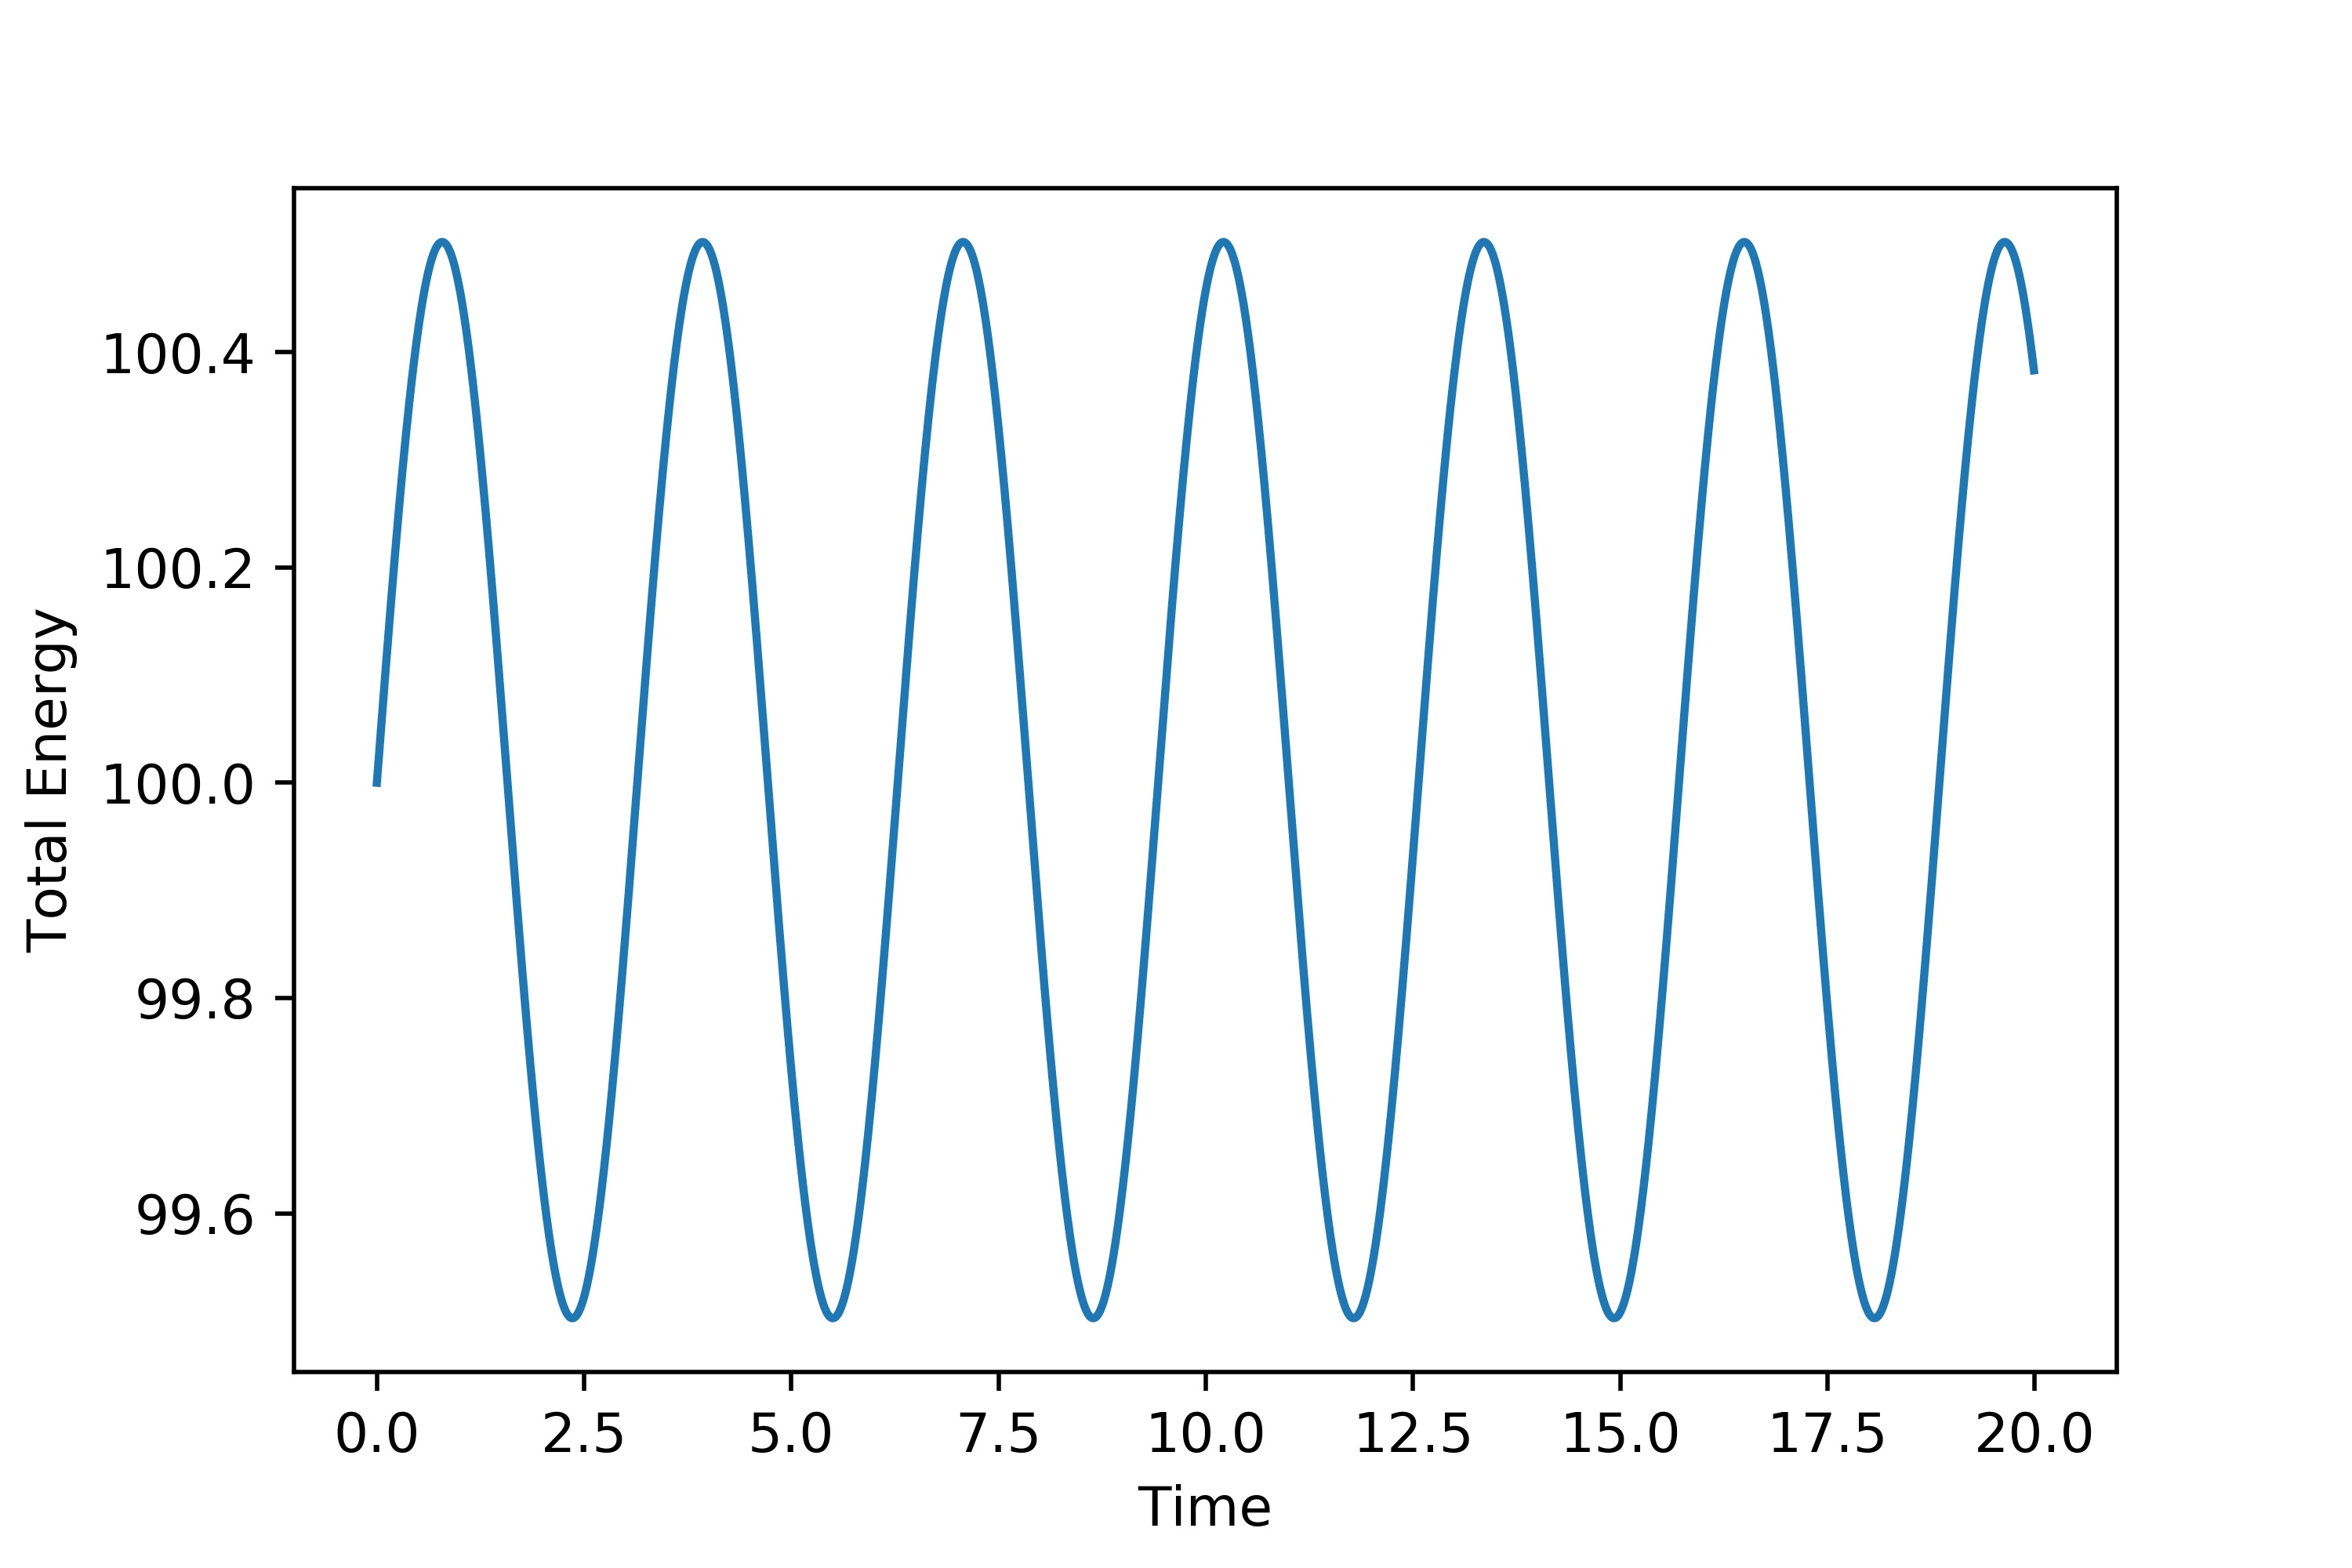
\includegraphics[width=\textwidth]{TE3.jpg}
\caption{Evolution of total energy over time for a simple harmonic oscillator modeled by the symplectic Euler method. Unlike the explicit and implicit methods, where the energy of the system monotonically increased or decreased (respectively), the energy here oscillates around the analytic system energy of 100. This is consistent to the phase-space manifestation of the symplectic method, since a conservation of phase-space area implies a conservation of average system energy.}
\end{figure}

\begin{figure}[H]
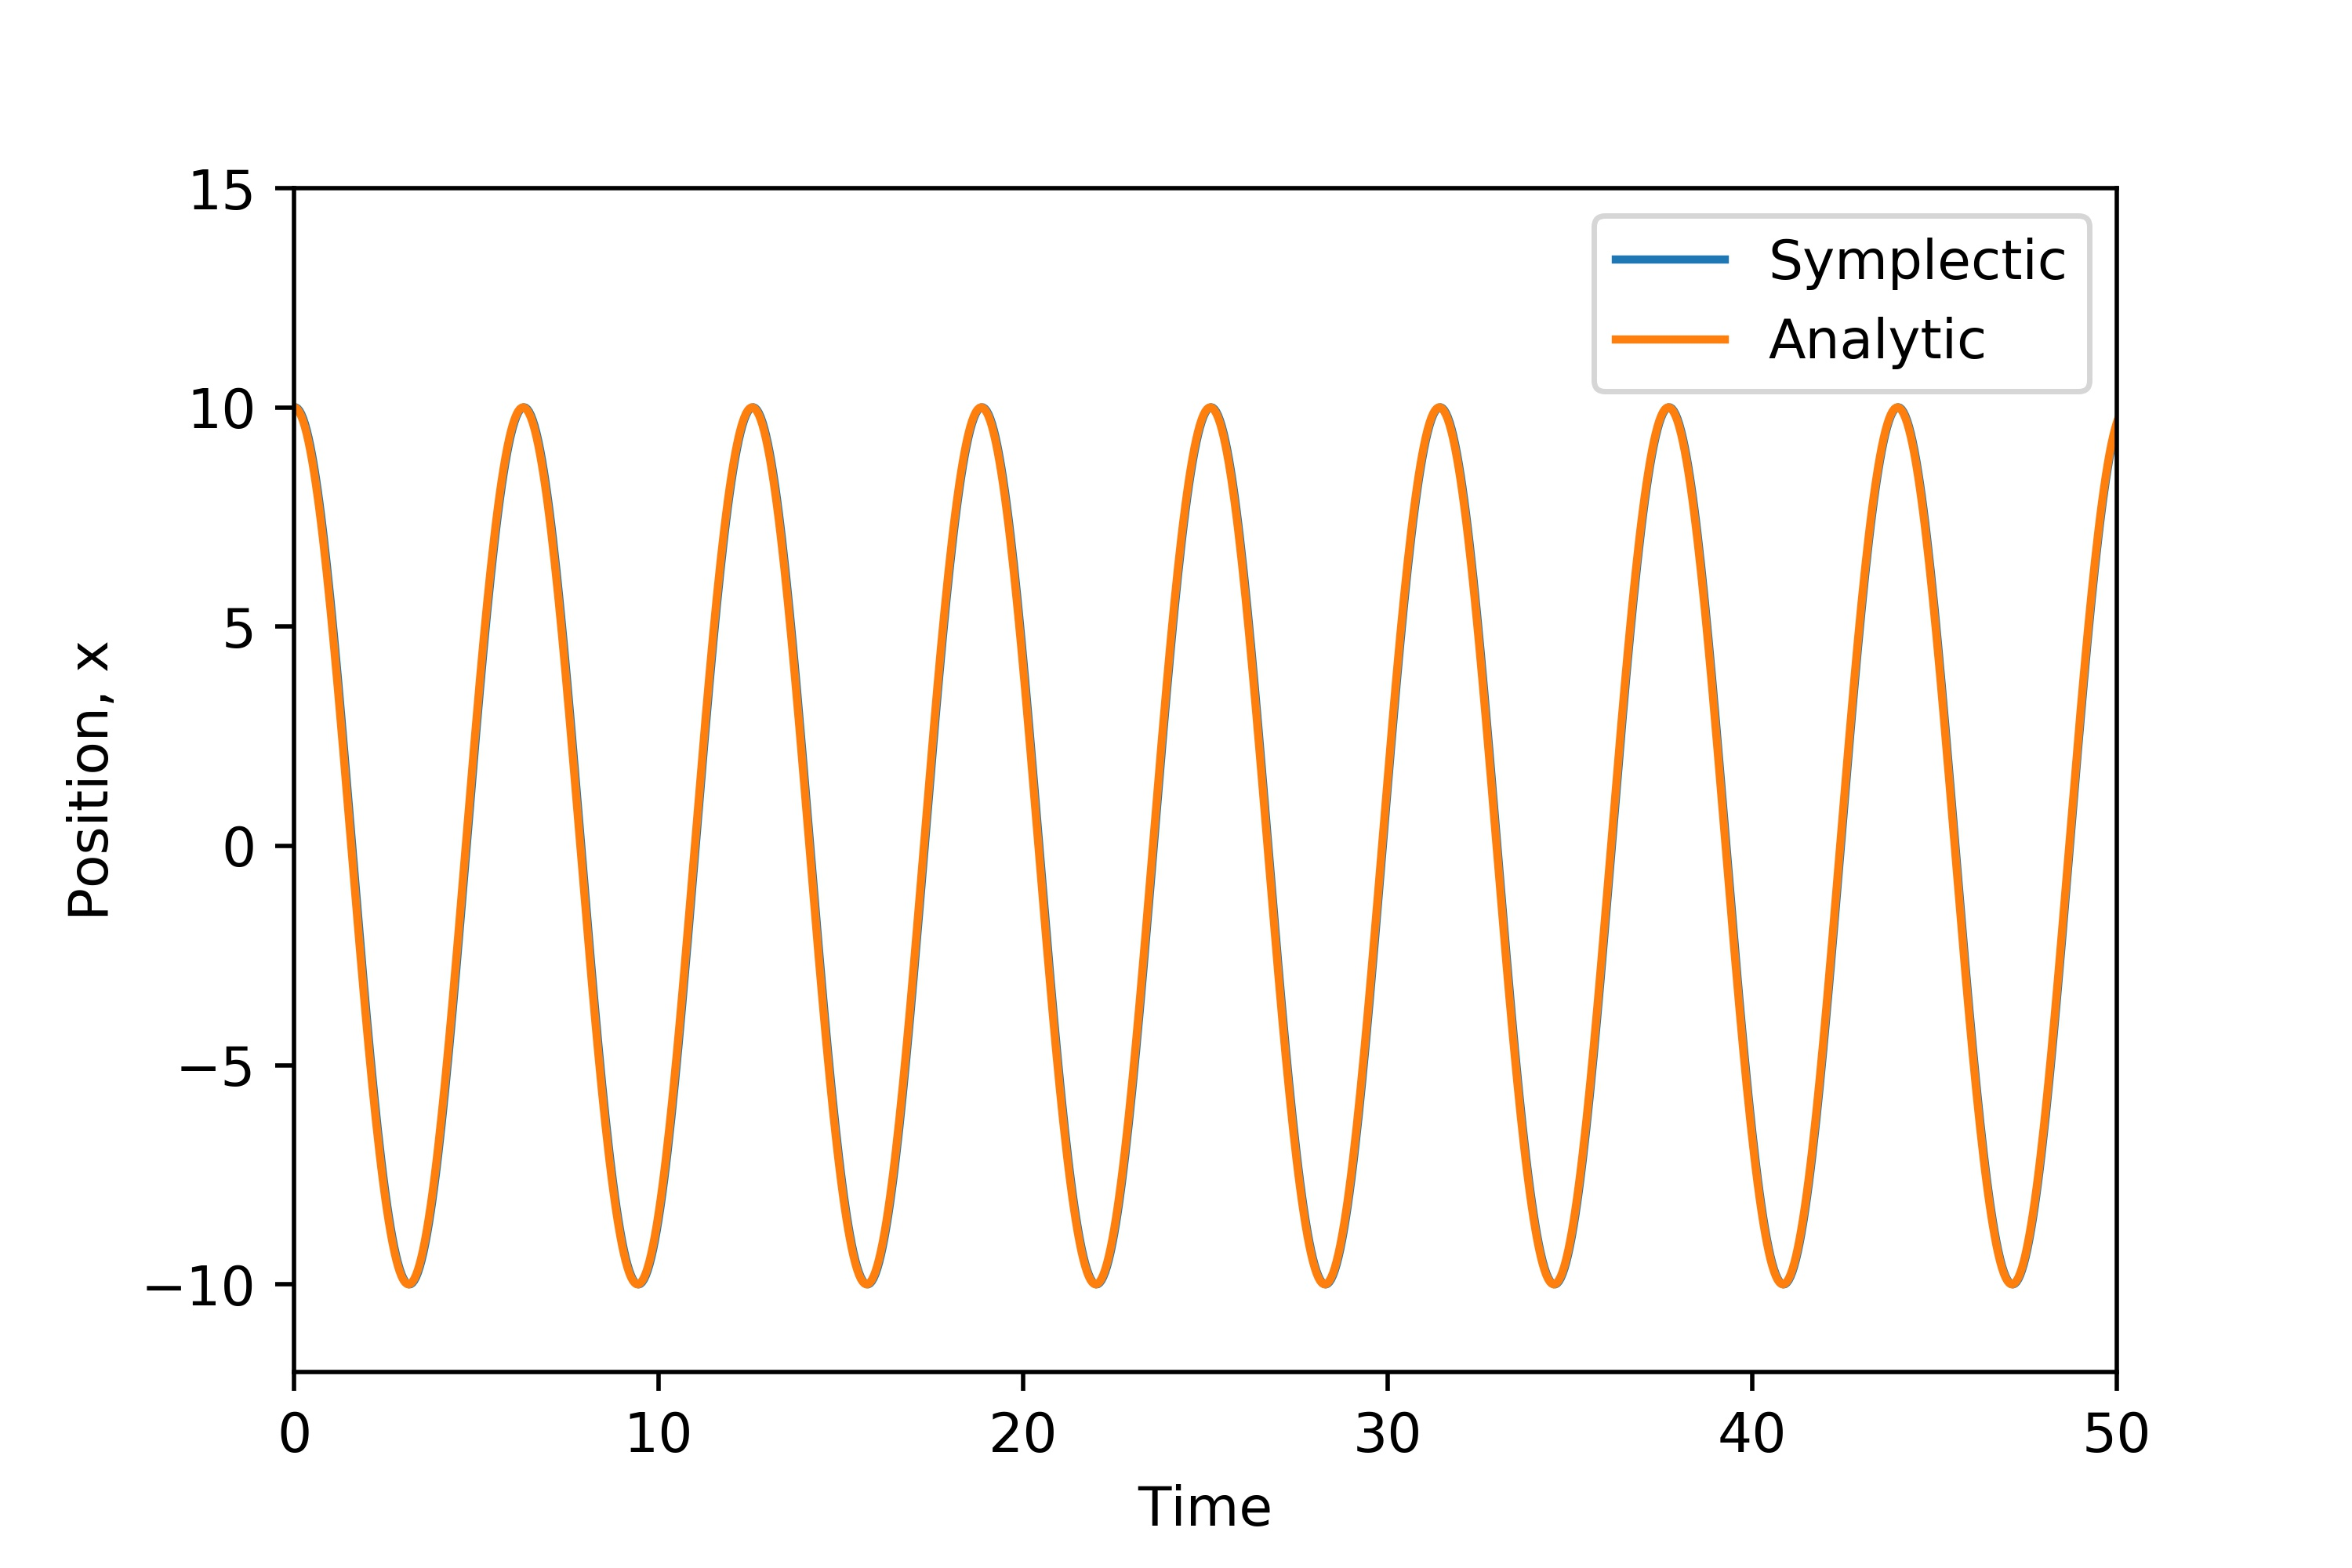
\includegraphics[width=\textwidth]{offset1.jpg}
\caption{Short-term comparison of low resolution ($h=0.05$) symplectic position with the analytic position. There appear to be no visible discrepancies on this time scale.}
\end{figure}

\begin{figure}[H]
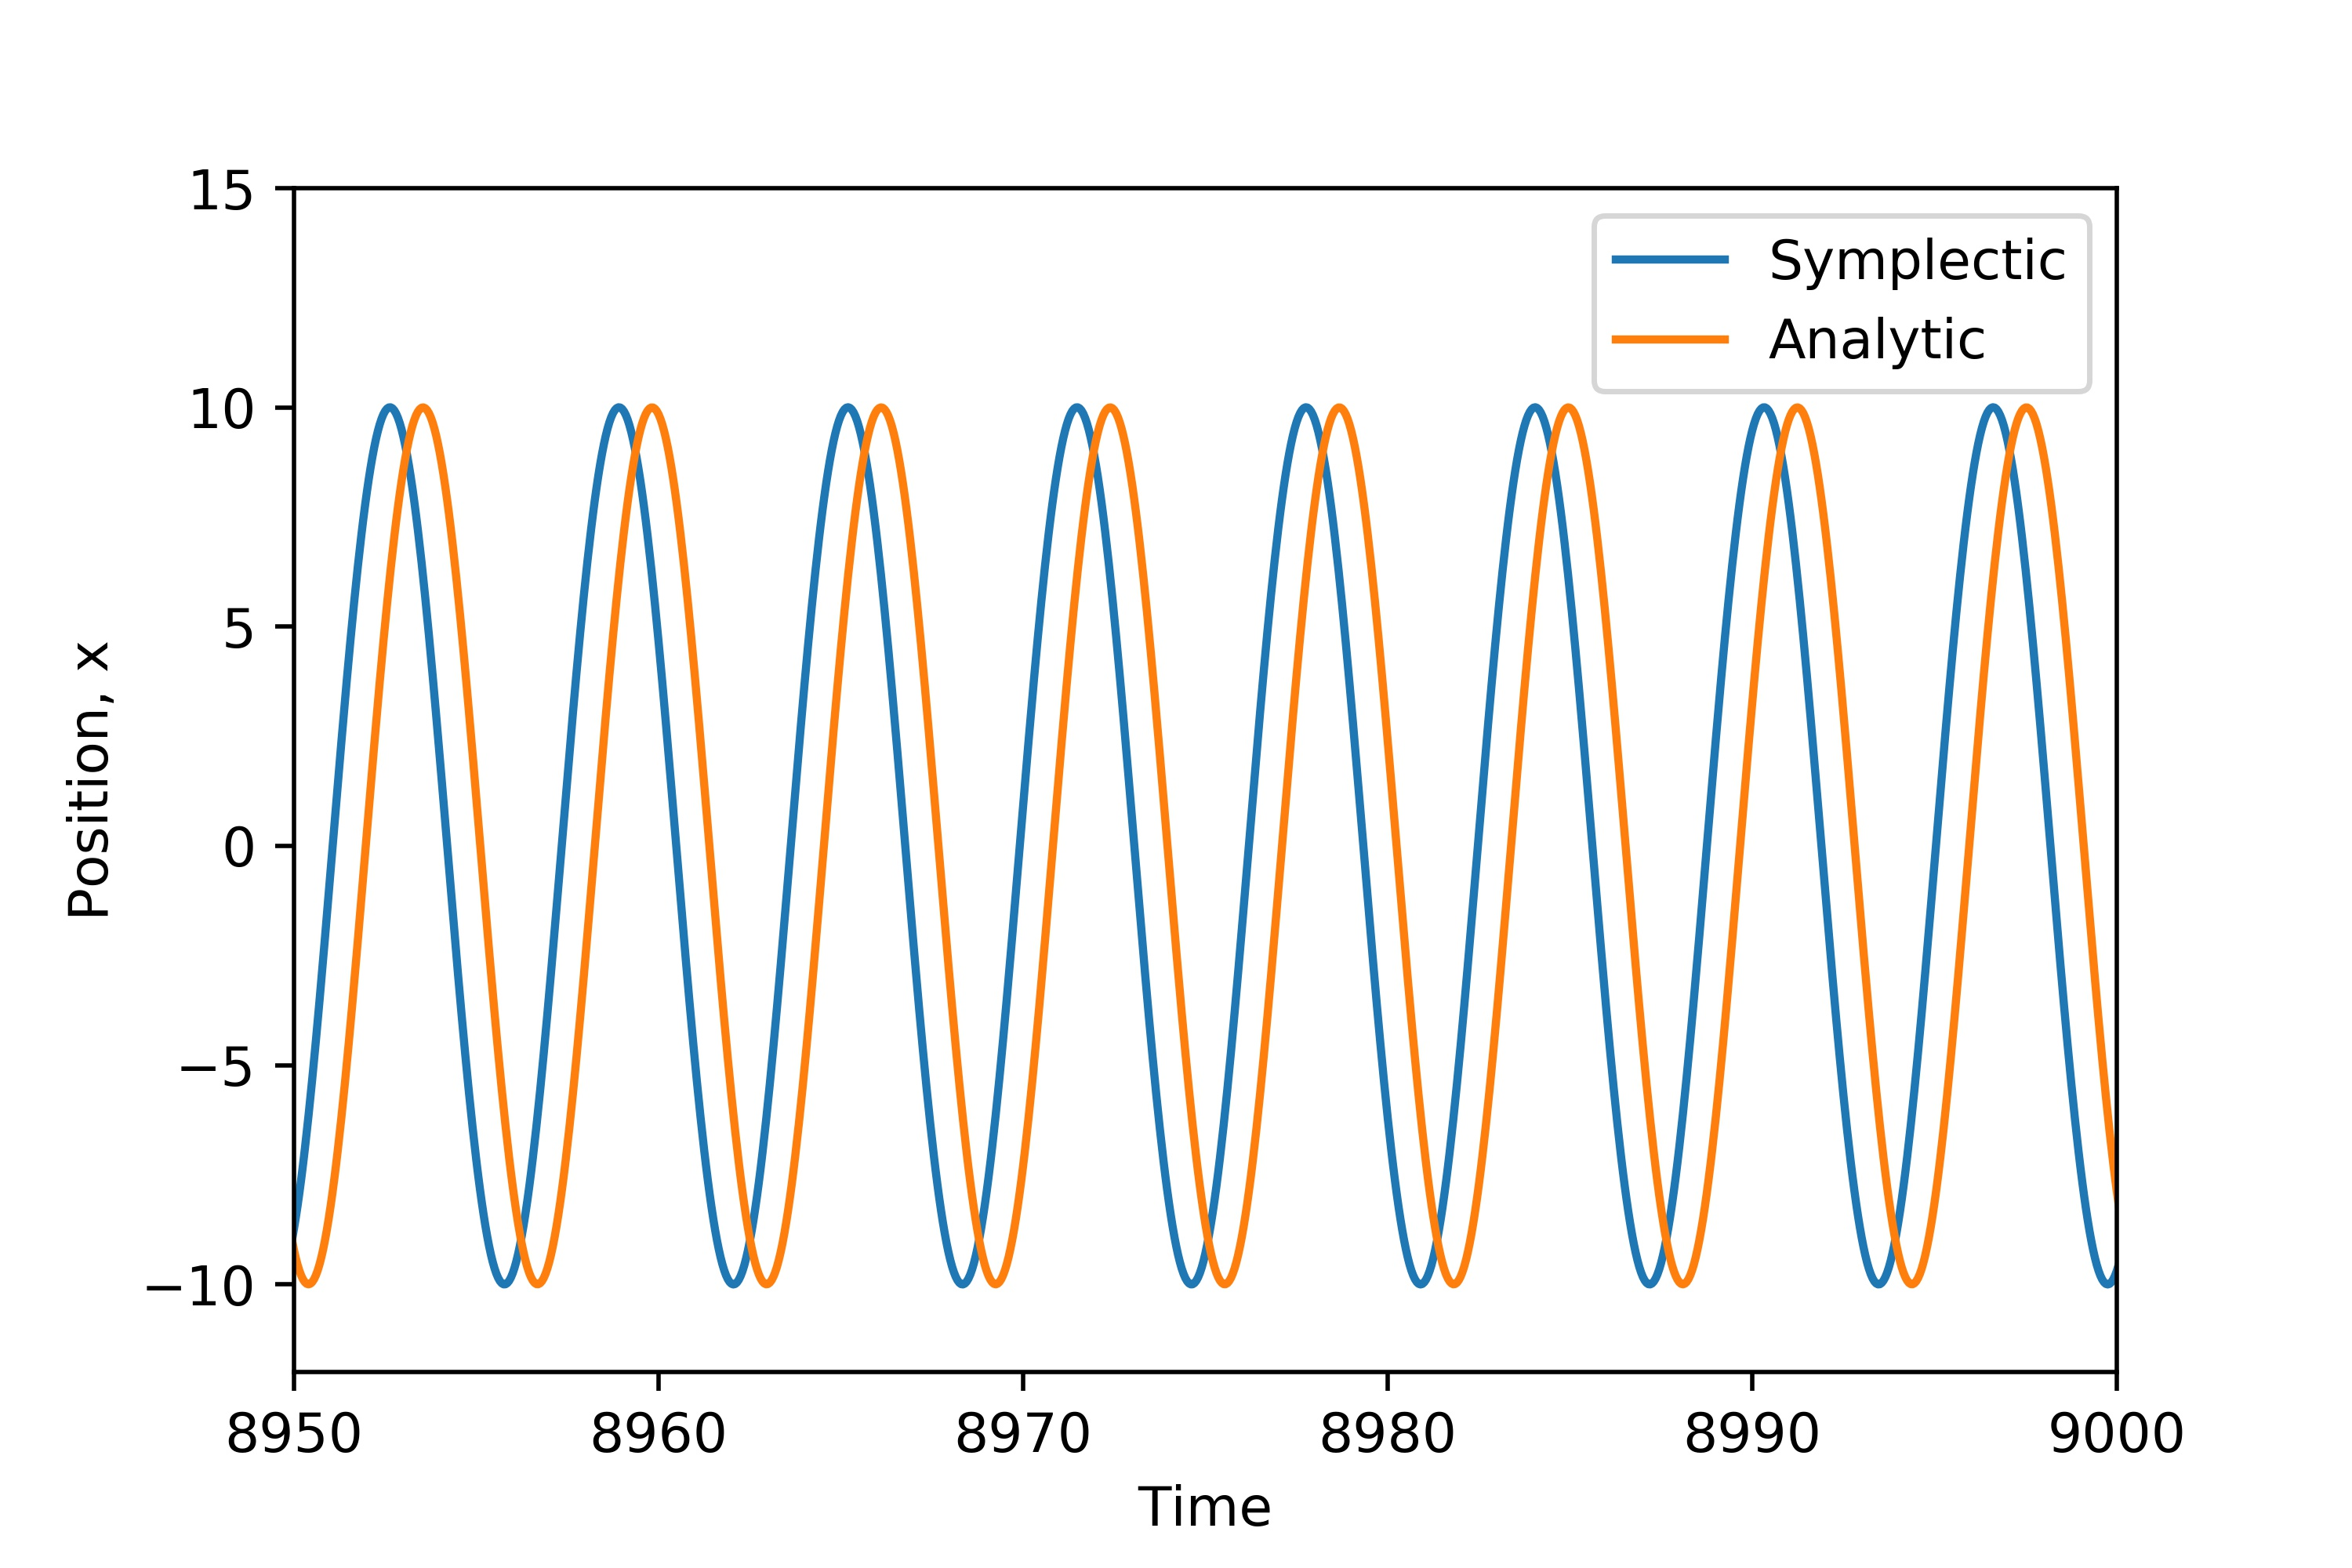
\includegraphics[width=\textwidth]{offset2.jpg}
\caption{Long-term comparison of low resolution ($h=0.05$) symplectic position with the analytic position. At these large times, there is a noticable phase lag of the symplectic curve, though the amplitudes of the symplectic and analytic position are equivalent.}
\end{figure}


\end{document}